\documentclass[a4paper,11pt,titlepage]{report}
\usepackage[a4paper,total={6in,9in}]{geometry}
\usepackage[skip=0pt plus1pt, indent=0pt]{parskip}
\usepackage[utf8]{inputenc}
\usepackage[T1]{fontenc}
\usepackage{utopia}
\ifdefined\HCode
	\usepackage[xindy,noautomatic]{imakeidx}
\else
	\usepackage[]{imakeidx}
\fi
\usepackage{tex4ebook}
\usepackage{ifthen}
\usepackage{fancyhdr}
\usepackage{lastpage}
\usepackage{graphicx}
\usepackage{xcolor}
\usepackage[hyperindex=true]{hyperref}

% Disable hyphenation
\tolerance=1
\emergencystretch=\maxdimen
\hyphenpenalty=10000
\hbadness=10000

% Avoid single lines on pages (widows/orphans)
\widowpenalty=10000
\clubpenalty=10000

% Replace "Chaper #" with "Album #"
\renewcommand{\chaptername}{Album}

% Remove lettergroups from EPUB index
\providecommand*\lettergroup[1]{}

% Make alphabetical song index (using style file)
\makeindex[intoc,name=songs,columns=3,title={Song Index},options={-s thebook.ist}]

% Make word index (using style file)
\makeindex[intoc,columns=2,title={Word Index},options={-s thebook.ist}]

% Setup title page
\title{\centering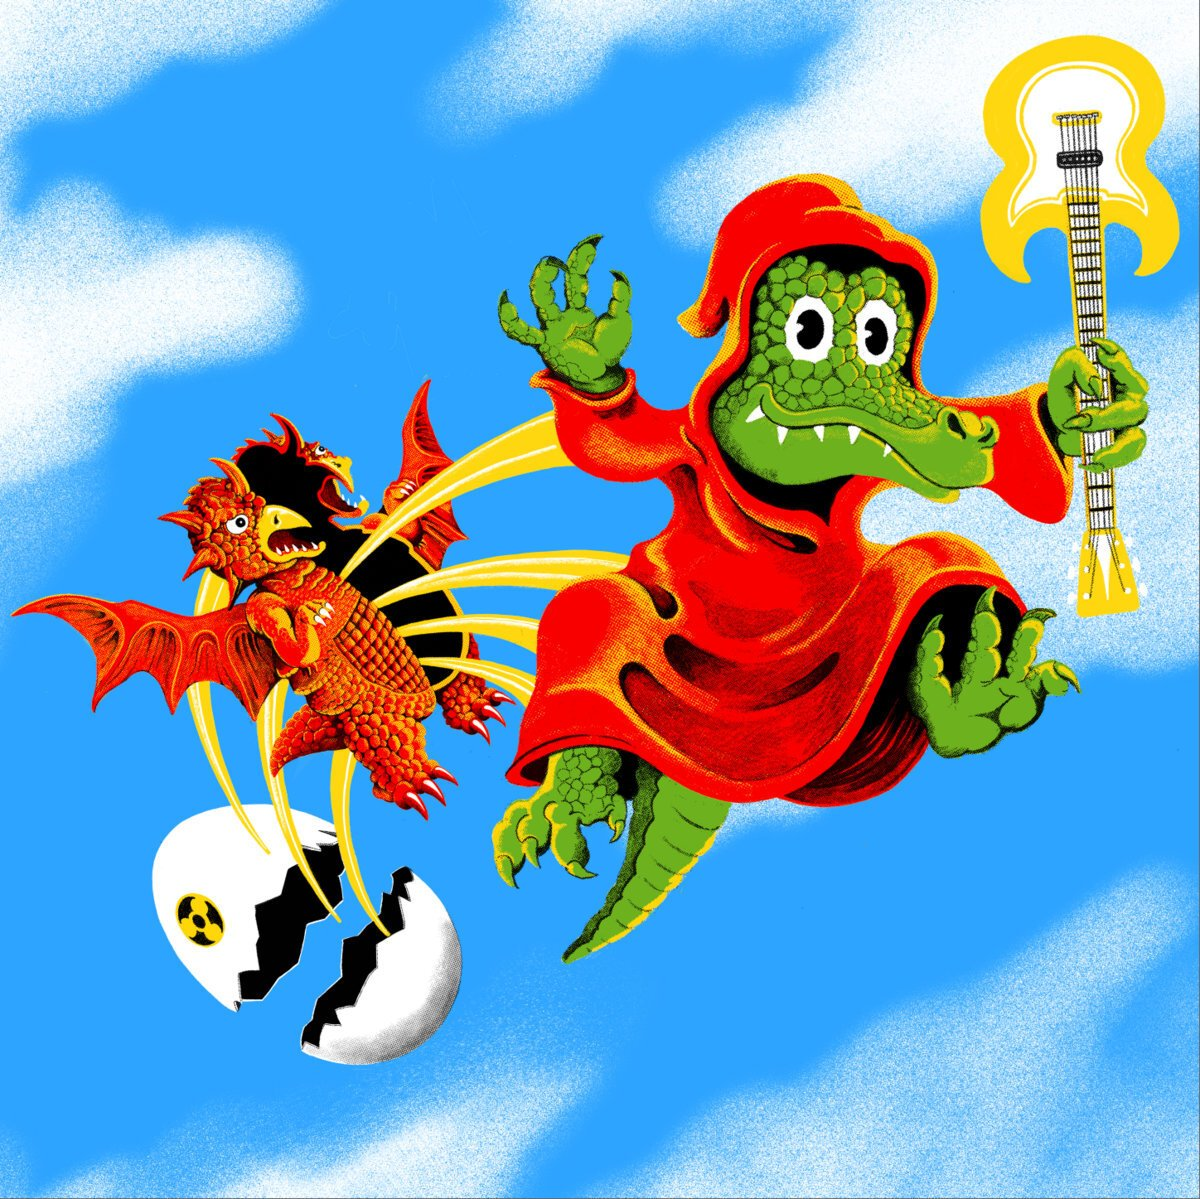
\includegraphics[width=0.8\linewidth]{cover-image.jpg}\\[1cm]%
    The Book\\{\large of Lyrics}} 
\author{King Gizzard \& the Lizard Wizard}
\date{\today}

% Adjust head height for fancyhdr
\setlength{\headheight}{14pt}
\addtolength{\topmargin}{-2pt}

% This must be here, because defaults are set and renewcommand for section marks will work.
\pagestyle{fancy} 

% Setup page headers/footers
\renewcommand{\chaptermark}[1]{\markboth{#1}{}}
\renewcommand{\sectionmark}[1]{\markright{#1}}
\fancypagestyle{plain}{%
   \fancyhf{} % clear all fields
   \renewcommand{\headrulewidth}{1pt}
   \lhead{\nouppercase{\leftmark}}
   \rhead{\nouppercase{\textit{\rightmark}}}
   \lfoot{}
   \cfoot{\thepage / \pageref{LastPage}}
   \rfoot{}
}%

%======================================================================

\begin{document}

% Define some shortcuts
\newcommand{\lindex}[1]{%
  \lowercase{\def\temp{#1}}%
  \expandafter\index\expandafter{\temp}%
}

\newcommand{\album}[1]{\chapter{#1}\vspace*{-1cm}}
\newcommand{\albumart}[1]{\begin{center}\includegraphics[width=4cm]{artworks/#1}\end{center}}
\newcommand{\song}[1]{\section{#1}\index[songs]{#1}}
\newcommand{\note}[1]{\emph{#1}\newline}
\newcommand{\word}[2][]{%
	\underline{#2}%
	\ifthenelse{\equal {#1}{}}%
	{\lindex{#2}}%
	{\lindex{#1}}%
}

% Make title page
\maketitle
\clearpage

\pagestyle{empty}

% Make frontmatter page
\begin{center}
{\relscale{0.8}%
\vspace*{\fill}%

This e-book collects all lyrics from the Australian band \emph{King Gizzard \& the Lizard Wizard}. \\[1em]
I started this project in June 2025 because I wanted to read Gizz lyrics on my e-book reader while listening to their music.
The included songs are grouped by album, and albums are added in chronological order (oldest first.)
There is also a song index at the end of the document that lists all songs in alphabetical order regardless of album,
and a word index that references selected words that are reoccuring throughout the lyrics. \\[1em]

Compiled by Jan Behrens (zykure). \\[1em]

This project is available on GitHub: \\
\href{https://github.com/zykure/KGLW-TheBook}{https://github.com/zykure/KGLW-TheBook} \\[2em]

All artwork and lyrics are copyright by \\
King Gizzard \& the Lizard Wizard and the respective authors. \\[2em]

\underline{Lyrics credits:} \\
Michael Cavanagh \\
Cook Craig \\
Lucas Harwood \\
Ambrose Kenny-Smith \\
Stu MacKenzie \\
Joey Walker \\[2em]

\underline{Artwork credits:} \\
Jason Galea \\[2em]

A big thanks to @michal-h21 for creating the TeX4ebook package: \\
\href{https://github.com/michal-h21/tex4ebook}{https://github.com/michal-h21/tex4ebook} \\[1em]

Shoutout to \\
\href{https://kglw.net}{\textit{kglw.net}}, \href{https://weirdoswarm.org}{\textit{weirdoswarm.org}}, \href{https://gizzheads.de}{\textit{gizzheads.de}} \\
and the Gizz global community! \\

\vfill%
}%
\end{center}


\clearpage

% Print table of contents
\tableofcontents

\pagestyle{plain}

% Add lyrics
\album{12 Bar Bruise}

%----------------------------------------------------------------------

\song{Elbow}

\note{[Written by: Stu MacKenzie]}

You want\\
You got\\
You are such a big shot\\
You cunt you know me better\\
Than to bend my elbow back\\
Stab me in the back\\

EY EY EY EY EY EY EY EY\\

%----------------------------------------------------------------------

\song{Muckraker}

\note{[Written by: Stu MacKenzie]}

Clear the cobwebs off my brain\\
Ants have came\\
It smells like rain\\

Pissin' shit off porcelain\\
I'll rake the muck\\
It's just my luck\\

Oh no, oh no\\
Muckraker\\

%----------------------------------------------------------------------

\song{Nein}

\note{[Written by: Stu MacKenzie]}

Never, never, never, never,\\
Had much too much, I'm sick of it\\
My body's full of poison shit\\
Never, never, well, ha ha, ha, ha!\\

Shit, never again\\

One, two, three, four, five, six, seven, eight\\
Nein! Nein! Nein! Nein! Nein!\\

%----------------------------------------------------------------------

\song{12 Bar Bruise}

\note{[Written by: Stu MacKenzie]}

Better be slave\\
Make some money\\
So when it gets ruff\\
We can bruise some stuff\\

But look at my dick\\
I bet you it's limp\\
Should I quit drink\\
It makes me think that…\\

12 bar booze is\\
12 bar bruise\\

Gotta be strong\\
Make me live long\\
Better not wait\\
For a bottle's sake\\

All of my friends are\\
Looking up dresses\\
They have not seen\\
The bruise that I've seen\\
Broo-oo-oo-oo-uize\\

%----------------------------------------------------------------------

\song{Garage Liddiard}

\note{[Written by: Stu MacKenzie]}

My head\\
Oh my head\\
My head's all bleak\\
And it makes my love so rough\\

My knees\\
Oh my knees\\
My knees are weak\\
And it makes for walking tough\\

Oww! Oww! Oww! Ouch!\\

%----------------------------------------------------------------------

\song{Sam Cherry's Last Shot}

\note{[Written by: Stu MacKenzie]}

Early that morning, the wagon-master of the train\\
came into the post greatly excited,\\
and reported that the dead body of a man and horse\\
had been found in the road about six miles from the post.\\

A company of infantry was immediately ordered out,\\
and proceeding to the spot found the body of Sam Cherry,\\
pinned fast to the ground by the dead body of his horse.\\

The search was continued, and in the lateral canyon were found\\
the bodies of Sargent Love and the three privates loaded with bullets,\\
mutilated and disfigured, but giving every evidence\\
of having sold their lives as great men should.\\

Trails were examined and the whole story worked out.\\

The party traveled along the road nearly to the entrance\\
of the canyon of the Limpia, known as the "Wild Rose Pass,"\\
when suddenly about thirty mounted Indians\\
dashed from the bushes along the stream,\\
cutting it off from retreat towards the Fort,\\
and driving it up the lateral canyon.\\

Suspecting a trap, Sam Cherry suddenly turned,\\
dashed through the line of Indians,\\
regained the road, and ran for life, away from the Fort,\\
followed by a number of yelling savages.\\

He was evidently doing well, when his horse stumbled and fell,\\
breaking his neck, and pinning Sam's leg to the ground.\\
In an instant he was surrounded by the exultant Indians.\\

Raising himself slightly, Sam fired five shots at his enemies,\\
then turning the muzzle against his own temple, he escaped\\
the tortures of their vindictive rage by his "last shot."\\
The baffled and terrified Indians went away as fast\\
as their ponies could carry them,\\
not touching the body,\\
not even taking the arms.\\

Such is the way out in the west.\\
People die by extreme barbaric ways.\\
But we're taking their land,\\
and in return they take our viscera\\
and spread it across the desert plains.\\

%----------------------------------------------------------------------

\song{High Hopes Low}

\note{[Written by: Stu MacKenzie]}

Well I ain't dumb\\
But I ain't that smart\\
And I can't spell\\
But I can sound it out\\

Gotta keep your high hopes low\\

%----------------------------------------------------------------------

\song{Cut Throat Boogie}

\note{[Written by: Stu MacKenzie \& Ambrose Kenny-Smith]}

As a child I felt inclined\\
To fold my ears in twine\\
Never once was I confined\\
I picked and choosed about my ride\\
So buckle me in before we set sail ahead\\
For it smells like cabbage\\
Got way too stale like death\\

Oh you're white as a ghost\\
I never felt so pale\\
As the blood dripped across the floor\\

So put it buried in your chest\\
With the rest of your drunken regrets\\
Inches from your jugular\\
As the room fills in front of ya\\
It took them long enough\\
For them to stop and suggest\\
Hey we better get him some help\\
We better get him out of here\\

How did I manage to cope as the blood soaked\\
Through my clothes and to the floor\\
From outside to the bathroom door\\
I was inches from my life\\
Yeah that's what keeps me up at night\\

Oh how did I survive / you shoulda died\\
How did I manage to cope / being alive\\
After all it was just a / innocent play fight\\
I hope they don't stop to sympathise\\

Stitch up the past to cure their whoremented heart\\

Tormented dreams it's all left in between…\\

%----------------------------------------------------------------------

\song{Bloody Ripper}

\note{[Written by: Stu MacKenzie]}

Push me down I will not crack\\
You're just a monkey with your claws in my back\\
I said it, and you heard\\
That murky bottle's cuttin' me some slack\\

But it's like all I wanna do\\
Sink my teeth in you\\
You already told me to\\
You said it's alright\\

%----------------------------------------------------------------------

\song{Uh Oh, I Called Mum}

\note{[Written by: Stu MacKenzie]}

Uh oh, uh oh\\
Uh oh, uh oh\\
Uh oh, uh oh\\
Uh oh, uh oh I called Mum!\\

I bought a funny glob\\
I put it in my gob\\
I had anxiety\\
I couldn't help myself\\
But call Mum\\

%----------------------------------------------------------------------

\song{Sea of Trees}

\note{[Written by: Stu MacKenzie]}

Oh hell I'm feeling underwater\\
My head is sinking like a stone\\

And hell I'm feeling kinda sick / like a prick\\
I don't know what's the use in it\\

And when you're feeling suicidal\\
Sometimes you've just got to unfold\\

%----------------------------------------------------------------------

\song{Footy Footy}

\note{[Written by: Stu MacKenzie \& Joey Walker]}

Footy footy\\
All I wanna do is\\
Footy footy\\
All I wanna kick is\\
Footy footy\\
Catch the ball, kick play on!\\
Crumb the ruck, run, handball!\\
Footy footy\\
Footy! Footy! footy!\\

Ang Cristou, Che Cockatoo-Collins,\\
Phillip Matera, Gavin Wanganeen,\\
Gary Moorcroft, Aussie Jones,\\
Bruce Doull The Flying Doormat,\\
Spider Everett, Spider Burton,\\
Craig Bradley,\\
The 1995 Carlton football team\\

Footy footy\\
Footy footy\\
Footy footy\\
Footy footy\\

Diesel Williams, Dale Kickett,\\
Sticks Kernahan, Darren Jarman,\\
Chad Rintoul, Ashley Sampi,\\
Mick Martin, Clint Bizzell,\\
The Brisbane Bears,\\
Aaron Hamill, everyone…\\

I'm gonna go down to Waverley Park\\
I'm gonna sit on the wing\\
I'm gonna eat a pie\\
I'm gonna buy a footy record for a dollar fifty\\
I'm gonna have a full strength beer ya girl\\
I'm gonna take a specky\\
I'm gonna kick a banana\\
I'm gonna eat a banana\\
I am gonna love every second of it\\
I hate what this game has become.\\

% ...
\album{Laminated Denim}

\artwork{laminated-denim.jpg}
\released{2022}{10}{12}
\label{album:laminated-denim}

%----------------------------------------------------------------------

\song{The Land Before Timeland}

\writtenby{Mackenzie/Cavanagh/Craig/Kenny-Smith/Walker}

\vocalsby{Stu Mackenzie}

It's good to be back. \\
Re-railed. \\
Back on track. \\
Change the clock through sleight of hand. \\
The \word{river} has been spanned. \\
Behold: the land before Timeland. \\

Teleportality. \\
Teleport you and me \\
From possibility to actuality. \\
Denim laminated. \\
Past illuminated. \\
Evil stimulated. \\
Future pixelated. \\

Laminated denim. \\

Laminated denim. \\
\word{Rattlesnake} venom. \\
\word{Serpent}-man demon. \\
Laminated denim. \\
Hide-out in the plenum \\
Where they can't get us. \\
Warmer air can benumb. \\
Laminated denim. \\

Laminated denim. \\
The forces came to hem in. \\
They'll get in if we let them. \\
Laminated denim. \\
Sunrise gameplan. \\
\word{Sky} like a lemon. \\
In \word{death} I'll be \\
A free man or woman. \\
Laminated denim. \\

It's good to be back. \\
Re-railed. \\
Back on track. \\
Change the clock through sleight of hand. \\
The river has been spanned. \\
Behold: the land before Timeland. \\

Teleportality. \\
Teleport you and me \\
From possibility to actuality. \\
Denim laminated. \\
Past illuminated. \\
Evil stimulated. \\
Future pixelated. \\

Laminated denim. \\

Laminated denim. \\
Satanic journeyman. \\
Seven metre wingspan. \\
Laminated denim. \\
Fire-winds are blowing. \\
Hourglass is going. \\
Long nights are impending. \\
Laminated denim. \\

It's good to be back. \\
Re-railed. \\
Back on track. \\
Change the clock through sleight of hand. \\
The river has been spanned. \\
Behold: the land before Timeland. \\

%----------------------------------------------------------------------

\song{Hypertension}

\writtenby{Mackenzie/Cavanagh/Craig/Kenny-Smith/Walker}

\vocalsby{Stu Mackenzie}

Like a red herring, \\
Laminated denim. \\
A note outside the scale from beyond the pale. \\
Unwitting host, \\
Inside-out ghost. \\
Harbinger of changes, \\
Destiny exchanges. \\
Time slows, \\
Eyes close. \\
In crimson tubes the pressure grows. \\
Sticky red \word{death}, \\
Life theft. \\
\word{Hypertension} is all that's left. \\

Golden hour turns to pink vein wine light. \\
\word[satan]{Satan's} son, \\
Foul one. \\
Demon of time. \\
Bat wing membrane \\
Eclipsed the \word{Sun} for fun. \\

Generation ferry, \\
Laminated denim. \\
Rotate anti-clockwise \\
And see through backward facing eyes. \\
Feel its allure, \\
History jeweller. \\
Stumbled on its ladder \\
And eaten by its chasm. \\
Then your mind slows, \\
Stress grows. \\
In crimson tubes the pressure grows. \\
Sticky red death, \\
Life theft. \\
Hypertension is all that's left. \\

Who am I if not the \word[canary in coal mine]{canary in the coal mine}? \\
I won't be back. \\
I slipped and fell into its lap, \\
Innards boil inside my tracts. \\

I caught that hypertension in another dimension. \\
Inside my time invention, I've laminated denim… \\

\album{Changes}

\artwork{changes.jpg}
\released{2022}{10}{28}
\label{album:changes}

%----------------------------------------------------------------------

\song{Change}

\writtenby{Mackenzie/Kenny-Smith/Walker/Craig}

Who should we please? \\
Who's to believe? \\
Who should we change for? \\
Who could we be? \\
When my race is done, how did I run? \\
Did I par the course and pass the baton on? \\

Vote with your feet. \\
Make company. \\
Form a military of peace and kill the king. \\
Be a citizen of planet \word{Earth}. \\
Be a bigger man or woman 'cause we all can change. \\

Change. \\
Change… \\

Change for its own sake. \\
Uniformity gave me a belly ache. \\
I want a mutiny. \\
My mind is finally awake. \\
Who could we be given equal opportunity? \\
What could we see given equal chance to actually see change? \\

Change. \\
Change… \\

Is this what we consider changing for the better? \\
Maybe. \\

Is this what we consider changing? \\
Ah, save me. \\
Is this what we consider changing for the better? \\
Maybe. \\
Is this what we consider changing? \\

I'm changing. \\
I'm changing. \\
Is this what we consider changing for the better? \\
Maybe. \\
Is this what we consider changing? \\
Change… \\

Is this what we consider changing? \\
I'm changing. \\
I'm changing. \\
Is this what we consider changing? \\

We're changing pace. \\
Higher stakes. \\
So called heroes wearing fake capes. \\
Critically acclaimed. \\
Clinically deranged. \\
Push the buttons. \\
Keep on frontin' 'til they hear the thumpin' \\
Something's coming up the hallway out of the left field lane. \\
Hey. \\
My stomach's turning from the vermin up-skirt observing power hungry. \\
Tryna draw the curtains from the public person. \\
But there ain't no slicker villain that's deserving a serving on the killing floor. \\
Put 'em on the chopping board for all to see. \\

I'm like a sniper hiding in the tower. \\
I'm picking them off one by one. \\
Gateway drug to the only solution. \\
Cutting out their tongues before they jump the gun. \\
I'm the like the cupid trying bring the love but you keep getting out of my range. \\
No strings on my bow with broken arrows. \\
Running low on ammo to make a change. \\

Buildings that you know. \\
People come and go. \\
Are a certain way. \\
Always are the same. \\
And then you get the news that obliterates your view. \\
Amputate your truths. \\
The significance has changed. \\

Hospital inane. \\
Meaningless and grey. \\
But lie within the walls and the significance will change. \\
What would it take for us to change the game? \\
Maybe our existence is significance in vain. \\
The significance has changed. \\
Maybe our existence is significance in vain. \\

Buildings that you know. \\
People come and go. \\
Are a certain way. \\
Always are the same. \\
And then you get the news that obliterates your view. \\
Amputate your truths. \\
The significance has changed. \\

Hospital inane. \\
Meaningless and grey. \\
But lie within the walls and the significance will change. \\
What would it take for us to change the game? \\
Maybe our existence is significance in vain. \\

What would it take to build an ark for me and my friends? \\
Escape this old place with all that creeps and fish in the sea. \\
And all that flies and all the bugs inside of me. \\
Take all the good things and leave the \word{human} beings. \\

Da da da da da da da da… \\

Burnin' up. \\
Burnin' up. \\
Burnin' up. \\
Burnin' up now. \\

Change. \\
Change… \\

%----------------------------------------------------------------------

\song{Hate Dancin'}

\writtenby{Mackenzie/Kenny-Smith}

I still hate dancing. \\
Oh I still hate dancing. \\
I still hate dancing. \\
Oh I still hate dancing. \\

Whatever you say. \\
Whatever you don't say. \\
Whatever you say to me won't sway me. \\

She's coming straight for me. \\
The world's frozen. \\
I'm sweating. \\

I still hate dancing. \\
Oh I still hate dancing. \\
I still hate dancing. \\
Oh I still hate dancing. \\

Slow-mo at the disco. \\
And she's putting out her hand to tango. \\
Oh no! \\
Her hips are too close for comfort. \\
Now I'm losing control of myself. \\
What the hell is coming over me right now. \\
I feel like I'm about to freak out from the waist down. \\
No more caring about what other people think. \\
Let 'em kick up a stink. \\

I might like dancing. \\
Oh I might like dancing. \\
I might like dancing. \\
Oh I might like dancing. \\

Whatever you say. \\
Whatever you don't say. \\
Whatever you say to me is gonna swing me. \\

I was just joking. \\
I love it. \\
I was just kidding. \\
I love it. \\

I feel like dancing. \\
Oh I feel like dancing. \\
I feel like dancing. \\
Oh I feel like dancing. \\
I feel like dancing. \\
Oh I feel like dancing. \\
I feel like dancing. \\
Oh I feel like dancing. \\
I feel like dancing. \\
Oh I feel like dancing. \\
I feel like dancing. \\
Oh I feel like dancing. \\

%----------------------------------------------------------------------

\song{Astroturf}

\writtenby{Mackenzie/Cavanagh}

Everything's dead here. \\
Covered with plastic. \\
Everything's fluro. \\
Evergreen matter. \\
Gotta stop grass growin' \\
Cover that wormhole. \\
Gotta stop birds from shitting on my lawn. \\
When it don't matter everything's better. \\
Throwaway plates are better for business. \\
Everything's easy. \\
Better for the \word{Earth} is astroturf. \\

Six \word[butterfly]{butterflies} fluttered by. \\
Looked horrified. \\
``I just hatched from chrysalis. \\
I've only hours, 36. \\
I need a mate to do my biz and this is where I will die. \\
Heartbreaking way to end. \\
I will cry on astroturf.'' \\

Suitable texture. \\
Suitable color. \\
Miniature forest. \\
Better than nature. \\
Make me feel better knowing I won't go out. \\
On my lawn and see an animal. \\
Everything's sterile. \\
Even infertile. \\
Proud of my monster. \\
It's never been straighter. \\
Dog shit \word{heaven}. \\
Better than the Earth. \\
It's astroturf. \\

Six butterflies fluttered by. \\
Looked horrified. \\
``I just hatched from chrysalis. \\
I've only hours, 36. \\
I need a mate to do my biz and this is where I will die. \\
Heartbreaking way to end. \\
I will cry on astroturf.'' \\

Astroturfing. \\
Astroturfing. \\
Astroturfing… \\
Better than the Earth is astroturf. \\

Six butterflies fluttered by. \\
Looked horrified. \\
``I just hatched from chrysalis. \\
I've only hours, 36. \\
I need a mate to do my biz and this is where I will die. \\
Heartbreaking way to end. \\
I will cry on astroturf.'' \\

%----------------------------------------------------------------------

\song{No Body}

\writtenby{Mackenzie}

I floated up and for the first time I could relax and unplug. \\
My friend, it felt good. \\

To shuffle off this mortal coil. \\
To rise like oil in water. \\

To be not real. \\
To have no \word{soul}. \\
To have no body. \\

I woke to an eye-adjusting fright. \\
Baptised in the light and found myself in purgatory white. \\
Dead again in the void. \\

What was the lesson, \word{God}?
No, no, no, no body… \\
Are you real or not? \\
No, no, no, no body… \\

In \word{death} I know \word{life} was a hallucination. \\

%----------------------------------------------------------------------

\song{Gondii}

\writtenby{Mackenzie}

\word{Human} being domesticated. \\
\word[gondii]{Gondii's} in the amygdala. \\
Human being contaminated. \\
Living-murdered feline worshiper. \\

What it feels like is it feels like it's \word{dream}-like. \\

Can't get a message to my brain. \\
I can't control myself. \\
Can't get a message to my brain. \\
I can't control myself anymore. \\

What it feels like is it feels like it's dream-like. \\

Human being manipulated. \\
Gondii drizzles serotonin. \\
Human being lubricated. \\
Drowning in oxytocin. \\

Can't get a message to my brain. \\
I can't control myself. \\
Can't get a message to my brain. \\
I can't control myself anymore. \\
I've got oocysts inside my head. \\
I can't control myself. \\
Can't get a message to my brain. \\
I can't control myself anymore. \\

So am I the bird or am I the worm? \\
Do have I free will? \\
Do have I free thought? \\

Am I the chicken or am I the egg? \\
Have I liberty? \\
Have I my wings? \\

You shouldn't fight it or deny it. \\
Just breathe in and embrace it. \\
Symbiotic Gondii choir sings a song of fuzzy minds. \\

So am I the dog or am I the cat? \\
No, it's neither one. \\
I am the \word{rat}. \\

Can't get a message to my brain. \\
I can't control myself. \\
Can't get a message to my brain. \\
I can't control myself anymore. \\
I've got oocysts inside my head. \\
I can't control myself. \\
Can't get a message to my brain. \\
I can't control myself. \\

%----------------------------------------------------------------------

\song{Exploding Suns}

\writtenby{Mackenzie/Kenny-Smith}

Exploding golden \word{Sun}. \\
Bursting radiation. \\
Get on your feet and run for the shelter. \\
A change is gonna come. \\
8 minutes and 20 seconds. \\
Over before begun. \\

And all that was green is fire and dust. \\
And all that was blue has dried up. \\
And all that we knew has dropped off the edge of waterfalls. \\
What's after \word{Armageddon}? \\

Giant star. \\
A thousand tears. \\
Liquid \word{Moon}. \\
A billion years. \\
Music of the brightest spheres. \\
A gong for remodelled frontiers. \\
Vibrates like the string of time. \\
Dissonant storyline. \\
The past and future intertwine. \\
The sun explodes at any time. \\

Exploding sun erupts. \\
Causing deadly destruction. \\
The time has come. \\
Redux. \\
Final endgame. \\
A burning fireball. \\
No more white dwarf. \\
Our sins to be absolved. \\

And all that was green is fire and dust. \\
And all that was blue has dried up. \\
And all that we knew has dropped off of the edge of waterfalls. \\
What's after Armageddon? \\

Giant star. \\
A thousand tears. \\
Liquid Moon. \\
A billion years. \\
Music of the brightest spheres. \\
A gong for remodelled frontiers. \\
Vibrates like the string of time. \\
Dissonant storyline. \\
The past and future intertwine. \\
The sun explodes at any time. \\

The sun explodes at any time… \\

%----------------------------------------------------------------------

\song{Short Change}

\writtenby{Mackenzie}

Who should we please? \\
Who's to believe? \\
Who should we change for? \\
Who could we be? \\
When my race is done, how did I run? \\
Did I par the course and pass the baton on? \\

Change. \\
Change… \\

\album[Petrodragonic Apocalypse]{Petrodragonic Apocalypse;}
\vspace*{-.5\baselineskip}%
\textbf{or, Dawn of Eternal Night: An Annihilation of Planet Earth and the Beginning of Merciless Damnation}
\artwork{petrodragonic-apocalypse.jpg}
\released{2024}{06}{16}
\label{album:petrodragonic-apocalypse}

%----------------------------------------------------------------------

\song{Motor Spirit}
\note{[Written By: Mackenzie/Walker/Cavanagh/Craig/Kenny-Smith/Harwood]}

Oh holy rabble, we art ensnared to quiver liketh rippled air. \\
Diocese of did melt sand. \\
Worship with thy chroming hand. \\
Coal-black cloud horizon maketh landborn petromyzon. \\
Summon forth thy \word{motor spirit}. \\
Drink the fuckin' gas and killeth. \\

Light the fuel. \\
Propagate oxygen and heat. \\
Deify motor spirit. \\
Kiss goodbye the weak. \\

Oh holy frontier art unbound. \\
Thee kiss thy \word{God}. \\
I kisseth ground. \\
I holdeth flame yond burns at night. \\
A seraph of \word[isaiah]{Isaiah's} light. \\
Touch thy lips and purge thy skin. \\
Holy water. \\
Eyes within. \\
By thee, we sleep and die for you. \\
Ignite m'lord, we ride for you. \\

Motor spirit, motor spirit, motor spirit… \\

Black buckets everywhere brimming, spewing millionaires. \\
Rotting ancient zooplankton squashed below the megaton. \\
Sweet juice on my lips. \\
Motorised apocalypse. \\
See metal crunch and hear it. \\
Highway death by motor spirit. \\

Light the fuel. \\
Propagate oxygen and heat. \\
Deify motor spirit. \\
Kiss goodbye the weak. \\

High octane aviation. \\
Gasoline leak inhalation. \\
Paint chromer. \\
Broken home. \\
Bloody stool. \\
Gasket blown. \\
Pop the bonnet. \\
Oil check. \\
Fire-pious side effects. \\
Guarana drama. \\
Damage control. \\
Sniffing, huffing ethanol. \\

Motor spirit, motor spirit, motor spirit… \\

Dividing non-believers. \\
Fly my octane spirit weaver. \\

Burnt rubber. \\
Grave robber. \\
Fire starter. \\
Spark imparter. \\
Un-water. \\
Fun porter. \\
Sun mortar. \\
Manslaughter. \\
Motor spirit. \\
Don't fear it. \\
Buy a ticket. \\
Button flick it. \\
Kill the rigid. \\
Burn the bridges. \\
Pick the stitches. \\
Drink the riches. \\

Engine \word{Gaia}. \\
Piston wheeze. \\
The messiah on their knees. \\
Beg the wind. \\
Beg the tree. \\
Beg the bug for mercy. \\
Motor spirit. \\
Dragon race. \\
Burning cars. \\
Outer space. \\
Petrol king, abdicate. \\
Human-kind, exonerate. \\

Dire fate shall plague our land. \\
Hurricanes shall sweepeth sand. \\
The winds doth howl and moaneth. \\
Homes and lives overthrowneth. \\
But hark, brave occultists, bold. \\
Rise to save the world from cold. \\
Weaveth magic spells with care. \\
Banish the hellish nightmare. \\

Dance beneath the moon's bright glow as charms they work to and fro. \\
But alas, fire doth grown despite witches' ebb and flow. \\
Fires rage with wild intent destroying all they present. \\
The heat doth scorch the landeth. \\
Naught but ash in thy handeth. \\

End doth near. \\
We cannot hide as the earth doth shake and writhe. \\
Turn to sin with hearts sincere. \\
Block the way that led us here. \\

Motor spirit, motor spirit, motor spirit… \\

%----------------------------------------------------------------------

\song{Supercell}
\note{[Written By: Mackenzie/Walker/Cavanagh/Craig/Kenny-Smith/Harwood]}

Murder waits inside the wedge. \\
Sharpening it's sickle edge. \\
Spading forks. \\
Increasing spin. \\
Screaming tin. \\
Ruby slippers. \\
Tap ya heels. \\
In a spiral. \\
Orange peel. \\
Bodies flying on a rainbow. \\
Run Toto. \\
Lightning bites the jaws of hell. \\
Whip crack the tortoise shell. \\
Angle grinder, a welcome friend. \\
\word[dorothy]{Dorothy's} end. \\
'Tis best at night to stay afraid 'cos sirens sing a bombing raid. \\
Incant a blood-curdled yell. \\
Supercell. \\

Supercell. \\
Supercell. \\
The bombshell carousel raising hell. \\

Supercell absorbing structures. \\
Unforetold in biblical scriptures. \\
Throngs of livestock in the air. \\
Twisted stare. \\
Pickup trucks blown to pieces. \\
A rabble release faeces. \\
\word[god]{God's} dead on barren corn fields. \\
Prepare to yield. \\
Countless crushed cars on west main. \\
Hill of Gaash flooding with flame. \\
Rips bark from dying trees. \\
Tempest breeds. \\
The sky bleeds. \\
\word{Dragon} feeds. \\
The messiah on their knees. \\
Jupiter laughs immortal. \\
Supercell. \\

Oh, cruel fate that hath befallen us. \\
Oil-mad, spinning gaily in the tempest\

Supercell. \\
Supercell. \\
The bombshell carousel raising hell. \\

24 dead in my state. \\
Motor spirit subjugate. \\
Creator, a burning mouth. \\
Carnage north, east, west and south. \\
EF5. \\
Force of nature. \\
Demolition. \\
Meet your maker. \\
Throwing cities like leaves. \\
Our mortal surface is wiped clean. \\

Murdering everybody. \\
Careless of theology. \\
Good christians pummelled anon. \\
Agnostics, \word{Armageddon}. \\
History is in the eye awaiting death while leaders hide. \\
Futures locked by land and wind. \\
Garden of Eden chagrined. \\

Drowning wind. \\
Gasp for breath. \\
Plain snake. \\
Omen of death. \\
Drink the piss and smoke your meth. \\
No one left. \\

Supercell. \\
Supercell. \\
The bombshell carousel raising hell. \\

%----------------------------------------------------------------------

\song{Converge}
\note{[Written By: Mackenzie/Walker/Cavanagh/Craig/Kenny-Smith/Harwood]}

Lo, a sight most dire and bleak from yon celestial perch doth speak. \\
The earth shake. \\
The earth quiver. \\
As dazzling twisted pillars deliver. \\

Thank \word{god} for space and that I'm here. \\
The vacuum black. \\
The last frontier. \\
Grey snakes slither across country. \\
Magnetising and converging. \\

From the ISS, ungodly high, chaos madness evolves below nigh. \\
A tempest of great force and might. \\
A storm of such unparalleled fright. \\
The winds do howl. \\
The rains do pour. \\
The lightning strike. \\
The thunder roar. \\
The elements rage in wild excess. \\
A spectacle of cruel finesse. \\
Houses, cities, torn asunder. \\
The havoc wreaked, a sight to wonder. \\
May the lord have mercy on us all. \\
Pray the storm which risen, thus shall fall. \\

Trained forever to leave the ground. \\
The ruined garden. \\
Churning clouds. \\
Convergence be into the eye. \\
Storm dilates and people die. \\

Converge, converge, converge… \\
Storm surge. \\

I am removed. \\
I am a cloud. \\
In peering down, I am endowed. \\
\word{Motor spirit}, that brought me here. \\
Fly to the moon. \\
I have no fear. \\

The twisters worm as tyres burn. \\
The screeching rims. \\
Gale force winds. \\
The judgement day. \\
Murder tycoon. \\
Ground control from the birds eye view. \\

In wind tunnels stained red with blood. \\
All that was green to shit and mud. \\

Morphing twirling to single beast. \\
\word{Humanity}. \\
Tantalising feast. \\

Feast on blood of feckless. \\
Pull the tide like a blanket. \\

The storm is the aether. \\
Quintessence and preacher. \\
Aura drinker. \\
Spirit shrinker. \\
The one true \word{God}. \\
Vile smile. \\
'Mental yolks. \\
Nymphs, sylphs and pygmy's choke. \\
Drink the blood. \\
Tasting Tchort. \\
What hath God wrought? \\

Converge, converge, converge… \\

Hungry crawling fat grey rat snake seems faster than the speed of light. \\
Snail trail through the green glade. \\
Killer zig zags and flying kites. \\
Watching from the silence of space at lords converging in their place. \\
Generals destruction in wake. \\
Combining fronts. \\
Ultimate quake. \\

Mass destruction. \\
Challenging. \\
Human race unravelling. \\

Verily winds converge with force. \\
Deadly splendour over the course. \\
Immersed in a mouse trap for land. \\
Forever writ in nature's hand. \\
The land doth mourn. \\
The sea doth grieve. \\
For loss of life. \\
Destruction seen. \\
Verbose words fail to convey the horrors that this storm do slay. \\

Converge, converge, converge… \\

%----------------------------------------------------------------------

\song{Witchcraft}
\note{[Written By: Mackenzie/Walker/Cavanagh/Craig]}

In the fields once green and gold. \\
Where the summer's breeze was bold. \\
A supercell rages and roils. \\
Swirling vortex. \\
A bubble boils. \\
Witchcraft. \\
So upon one sable morn when the moon does wane and die. \\
A ragged coven convenes performing incantation nigh. \\
Witchcraft. \\
Taxidermy with eyes of fire. \\
Chanting songs above the lyre. \\
Miasma of hair and bile hangs heavy with the mother's ire. \\
Witchcraft. \\
Antlers shed ribbons of blood. \\
Draped like thorns upon the brow. \\
A crucifixion can end this squall. \\
A bible burned with aerosol. \\
Witchcraft. \\

I call upon the blood-moon goddess for I have but one request. \\
I've laid the altar. \\
Charged the crystals. \\
The circle, I have blessed. \\
Witchcraft. \\
The four elements are set. \\
Septuple trigger fingers bleed. \\
Oh horrors, my midnight god, what have you got in store for me? \\
Witchcraft. \\

Fire flickered and danced with hues of orange, red and deep burnt blues. \\
Snakes slither by, just out of sight. \\
Lizard and bat take wing in the night. \\
Around the fire, they circle slow and with locked minds a chant did grow. \\
Timbers of oak with knots so tight bear witness to spells cast in the night. \\

I am \word{Beowulf}. \\
I am cat, black. \\
Knock the candle from scripture stack. \\
I bring justice at moment, right. \\
\word{Gila} Monster, set alight. \\
Witchcraft. \\
Unleash a reptile thinking in terms of only \word{lizard} brain. \\
And be not lucky enough to make any mistakes again. \\
Witchcraft. \\
Like a grenade in a fist, the air ignites, a bloody mist. \\
Moon cycle shifting. \\
Demon lifting. \\
Beowulf, grifting ritualist. \\
Witchcraft. \\
Alas, the cat disrupts the prayer and turns it on meekest there. \\
The tiny creature, a harmless skink, transforms into a mythic king. \\
Witchcraft. \\

%----------------------------------------------------------------------

\song{Gila Monster}
\note{[Written By: Mackenzie/Walker/Cavanagh/Craig/Kenny-Smith]}

Anon, a giant monster roams. \\
Creature of magic, not of home. \\
He didst gobble each hag he found. \\
Screams didst echo, a chilling sound. \\
With every wiccan he will devour, he'll grow in strength, in size and power. \\
Until one day upon his back, he'll sprout wings. \\
A fearsome pack. \\
With each meal \word{Gila} grows more. \\
A biblical beast of ancient lore. \\
With fire in belly. \\
Flames in eyes. \\
The beast rise to the highest skies. \\
So beware, ye witches fair, lest thee be spied by \word{dragon}-glare. \\
It'll show not mercy, it is said, but devour thee and leave thee for dead. \\

Gila, Gila, Gila… \\
Monster. \\

I'm the Gila. \\
Blood spiller. \\
Witch killer. \\
Gila, Gila. \\
I'm the Gila. \\
Card dealer. \\
Fate sealer. \\
Gila, Gila. \\
I'm the Gila. \\
Blood spiller. \\
Witch killer. \\
Gila, Gila. \\
I'm the Gila. \\
\word{Godzilla} guerilla. \\

Diamondback climbing walls. \\
Puncture wounds. \\
Torn and mauled. \\
Raging monster. \\
Witch brawl. \\
Backlash. \\
Battlecry. \\
Curveball. \\
Pushed and probed to the edge. \\
No sense of forgiveness. \\
I'm the Gila. \\
The blood spiller. \\
The witch killer. \\
I'm the Gila. \\

Gila, Gila, Gila… \\
Monster. \\

Turncoat projectile. \\
Idiot reptile. \\
Born in the whirlwind. \\
Feral wonderkind. \\
Petty feline summoned anew. \\
Once was slave. \\
Master of you. \\
Abomination. \\
Hallucination. \\
Revenging sinner. \\
Witches for dinner. \\
I'm the Gila. \\
The card dealer. \\
The fate sealer. \\
I'm the Gila. \\

I'm the Gila. \\
Blood spiller. \\
Witch killer. \\
Gila, Gila. \\
I'm the Gila. \\
Card dealer. \\
Fate sealer. \\
Gila, Gila. \\
I'm the Gila. \\
Blood spiller. \\
Witch killer. \\
Gila Gila. \\
I'm the Gila. \\
Godzilla guerilla. \\

Growing immensely and vastly in size. \\
Summoned from the wicca to their demise. \\
Sprouting wings. \\
Demonic features. \\
Horny for bloodlust. \\
Lord of pagan creatures. \\
Blacker than space. \\
Its eyes are distant suns. \\
Devouring its disciples like mischievous sons. \\
In the forest of my mind runs a torrent of fire. \\
The real me beneath the liar. \\
I bide my time to don my crown. \\
Tasered bull. \\
Gore the clown. \\
Compared to me, a pulsar is a lighter flame. \\
Compared to mine, their wicca is a mere child's game. \\

Gila, Gila, Gila… \\
Monster. \\

My eyes feel like they're made of light. \\
Boötes void would be made bright. \\
I will blind you in the hadal zone. \\
Emperor of the abyss below. \\

Annihilation of planet \word{Earth} and the beginning of merciless damnation. \\

Oh, regret, what a cloud of dread. \\
With the cold hand of death ahead. \\
Oh, desperation, what a mind killer. \\
All hail, king Gila. \\

%----------------------------------------------------------------------

\song{Dragon}
\note{[Written By: Mackenzie/Walker/Cavanagh/Craig/Kenny-Smith]}

PetroDragonic Apocalypse. \\

Flapping wings weaving through. \\
Crocodile obsolete. \\
Flattened raze. \\
Spraying flames. \\
Blood curdle screech. \\

\word{Dragon}, dragon, dragon… \\

\word{Gila} is the aether. \\
Quintessence and preacher. \\
Aura drinker. \\
Spirit shrinker. \\
The one true \word{God}. \\
Vile smile. \\
Mental yolks. \\
Nymphs, sylphs and pygmy's choke. \\
Drink the blood. \\
Tasting Tchort. \\
What hath God wrought? \\

Dragon, dragon, dragon… \\

PetroDragonic Apocalypse. \\

Winged demon on the stratosphere is swooping beneath to kill with fear. \\
Stop the dragon, dragon, dragon, dragon. \\
Stop the dragon, dragon, dragon. \\
Scrambling jets and ballistic lies burned underneath the lidless eyes. \\
Stop the dragon, dragon, dragon, dragon. \\
Stop the dragon, dragon, dragon, dragon. \\
Atomic space. \\
Chaos, it reeks. \\
Pilots shriek. \\
Cities weep. \\
Stop the dragon, dragon, dragon, dragon. \\
Stop the dragon, dragon, dragon, dragon. \\
Dragon, dragon, dragon, dragon, dragon. \\
Stop the dragon. \\

The eye dilates. \\
The air gyrates. \\
A gate in the sky. \\
A portal to die. \\
A shriek from space. \\
A mangled yell. \\
Dragon descends. \\
Welcome to hell. \\

Audi mea verba. \\
Oh ignis draconis. \\
Ex cineribus orior. \\
Altius atque altius. \\
Alis patentibus. \\
Lumine micante. \\
Draco hic apparere debet. \\
In loco subter. \\

\note{[English translation:]}

{\itshape%
Hear my words. \\
Oh dragon fire. \\
From the ashes I rise. \\
Higher and higher. \\
With wings spread. \\
With a flashing light. \\
The dragon must appear here. \\
In a place beneath. \\
}

The eye dilates. \\
The air gyrates. \\
A gate in the sky. \\
A portal to die. \\
A shriek from space. \\
A mangled yell. \\
Dragon descends. \\
Welcome to hell. \\

Ex profunditate antiquae doctrinae. \\
Ad caelos supra semper. \\
Hoc incantamentum evoco. \\
Draco apparet. \\
Incantamentum iam transactum est. \\

\note{[English translation:]}

{\itshape%
From the depths of ancient learning. \\
To the heavens above forever. \\
I invoke this spell. \\
The dragon appears. \\
The spell is now cast. \\
}

A creature born of the tempest. \\
The thrill of the hunt. \\
The thrill of the quest. \\
A wild being of chaos and fire. \\
Knowing naught but it's own desire. \\
To taste fear in the game's eyes. \\
To claim it's victory. \\
To claim it's prize. \\
Killing all in its path. \\
Nay mercy shown. \\
Until the dragon stands triumphantly high-lone. \\

Dawn of eternal night, Dawn of eternal night, Dawn of eternal night… \\

Terra firma. \\
\word{Earth} murdered in the blink of an eye. \\
Malevolent equivalent. \\
Diabolify. \\
Bending storms beneath it's will. \\
Firelight troglodyte. \\
Dawn of eternal night. \\

Demonic bird reptilian desert fetid breath. \\
Sapien spite and fatal bite with a foul gas stench. \\
\word[isaiah]{Isaiah's} come to claim the throne. \\
The dragon's birthright. \\
Dawn of eternal night. \\

The beast we awoke hath been untamed. \\
Eyes of fireth and wings of a flame. \\
It hath arisen from chariest lair. \\
Spreading its wings and taking to the air. \\

Yeah. \\

%----------------------------------------------------------------------

\song{Flamethrower}
\note{[Written By: Mackenzie/Walker/Cavanagh/Craig/Kenny-Smith]}

Depths of hell. \\
\word{Dragon} rise. \\
Death in mind. \\
Smoking eyes. \\
Malice gleam. \\
Deadly guise. \\
Futile to hypothesise. \\
Soul blackened by the dark arts. \\
Strike a fear in mortal hearts. \\
Taketh to the sky with blazing darts. \\
Flame those foolish, lazy fucks. \\

My eyes start to spin. \\
Senses dulled by the original sin. \\
Newfound gasoline. \\
Sing and dance with thee. \\
My new family. \\
The folly of men. \\
The tragedienne. \\
A force of nature. \\
A force of might. \\
Fire on the land and wind in flight. \\
Those who stand before do cower in fright. \\
Oh fearsome one, thou art terrible sight. \\

Flame. Thrower. \\
Flame. Thrower. \\
Flame. Throw a flame. \\

Engage the mesolimbic pathway. \\
Stimulate brain reward activates. \\
Burn nerve numbing hot. \\
Swimming dopamine. \\
Sweet smelling, the flesh melting benzene. \\
Mouthfuls of the black bubbling fuel. \\
Feel it spray through the \word{lizard} nostrils. \\
Mayday, mayday! \\
Calling ground control. \\
The space station in a dragon-death-roll. \\

Flame. Thrower. \\
Flame. Thrower. \\
Flame. Throw a flame. \\

I drink lakes of motor oil. \\
I engulf and I inflame. \\
I disrupt the natural order. \\
I come of wind and I come of cloudburst rain. \\
I am the high priestess. \\
I spew motor spirit breath. \\
I will torch the \word{ISS}. \\
The last enemy to be destroyed is death. \\
Fire-pious church-goer. \\
Flamethrower. \\

Oil wells drained of fluids. \\
Underneath stand black gold druids. \\
The dragon turns his gaze above. \\
Releases his breath, a flaming dove. \\
Engines crunch on the ground below. \\
Through its teeth, cleansing lava flows. \\
\word{Gaia} set to self-destruct. \\
Flamethrower complacent fucks. \\

Motor spirit. Motor spirit. Motor spirit… \\

%----------------------------------------------------------------------

\song{Dawn of Eternal Night}
\note{[Written By: Mackenzie]}

The winds howled like ravenous wolves, clawing at the mansion's windows and doors. The sky had turned a murky shade of death, as if the clouds themselves were infected with the poison of a dying planet. The humans inside the mansion toiled like frenzied ants, their hands trembling as they performed ancient rituals in feverish synchronicity. Desperate to bend the forces of nature to their will, they attempted to tap into the wellspring of arcane, ritualistic magic. Foolish, in my opinion, but the humans had reached the brink of all possibilities; in their minds, only one remained. They hoped to wield their magic like a shield, protecting themselves from the deadly tornadoes that whipped over the land like whirling dervishes, collecting whole villages and tearing them asunder in the sky. The power they sought was shrouded in mystery, but the cause of the storms was clear. \\

\note{[First paragraph on lyric sheet, but not on song]}

The humans' terror and despair filled the room in a suffocating fog. Palpable, even to me, their pet \word{Gila} Monster. They frantically chanted and burned incense. Eyes, hearts and minds fixed on the swirling maelstrom beyond. They knew that time was slipping through their fingers, that the approaching storms were an unstoppable force, an untamed beast. Still, they persisted, their faith in the occult a tiny ember of optimism amid planet \word[earth]{Earth's} ashes of despair. As the winds grew louder and the mansion creaked and groaned, I knew their efforts were futile. The tornadoes were a force unlike any other, a manifestation of nature's rage and fury. A living fist of \word{God}. And no matter the strength of the humans' magic, it was but a flickering candle in the face of a raging inferno. \\

As darkness enveloped the mansion, the humans fervently performed rites, their voices a hymn pleading to ancient deities for deliverance. Dirty fingernails protruded from their robes, their eyes rimmed black from sleeplessness. Despite the vortex's tumultuous force, they persevered in their prayers and offerings. Desperate faith. Blind adherence. Collective insanity. The atmosphere in the room was heavy with the aroma of burning mugwort and myrrh, their voices a harmonic confluence of terror and desire, the monotony of their chanting ensnaring me in a hypnotic trance. I curled my tail around to lay my head upon it and relaxed. The old mansion quivered like a violin bow and the screaming of the wind turned to a sweet song. \\

As I lay in a fog of unconsciousness, my eyes locked with the house cat, \word{Beowulf}, who had been quietly watching from his perch atop a stack of sacred texts. Through the smoke of the mysterious herbs the humans were burning, Beowulf gave me a conspiratorial wink. Before I could decipher the enigmatic gesture, Beowulf stumbled and knocked over a candle, causing the flame to pirouette in the darkness. The humans seemed oblivious to the spilled candle, their focus fully absorbed in ritual. Eyes fixed on the altar and hands moved with graceful purpose as they wove their spells. But as the fire's tendrils creeped across the room like a snake roused from its slumber, it became clear that something was awry. The flames licked and hissed at the corners of the room, the fires hunger and intensity increasing with each passing moment. \\

I inhaled the smoke and felt an intense desire to be one with the fire. And so, I reached out and made contact. A strange energy coursed through my body. Something trembled within me like a \word{Kraken} stirring in its watery grave. An ancient dormant force. My body began to grow and change, my scales shimmering and shifting as I took on a new form. As the fire grew, so did I. My limbs elongated and new wings unfurled, my bones and muscles stretching and expanding to accommodate my new size. My head grew larger and \word{dragon}-like, my jaw widening and my teeth sharpening into deadly points. The fire raged but I didn't burn. I was a phoenix rising from the ashes, a butterfly emerging from its chrysalis. My body was a canvas, painted with brushstrokes of smoke and flame. I was a shape-shifter, a changeling, a being of endless potential. My skin was a cloak, shedding its old self to reveal a new, shimmering version. My eyes were windows to a vast, untapped universe. My mind was a labyrinth, a puzzle waiting to be solved. My heart was a forge hammering a new path forward. I was a being of fire and magic, a being of transformation and renewal. A rip in space-time. Born again. A force to be reckoned with. A being beyond human understanding. \\

The humans finally noticed the fire and my transformation taking place. Despite their fear, they continued to chant, their eyes wide with shock and confusion. Avatars to their gods. Something primal and formidable stirred within me, a force long slumbering, now roused. Profound and terrifying. The flames eagerly devoured me; I knew there was no turning back. Awe radiated from me and the humans saw it. It seemed their incantation had misfired; I was the materialisation of their mistake. They had never seen anything like this before, and their shock and disbelief was palpable. A tangible force in the air. What had gone wrong, I do not know; I paid them no mind. I was consumed by the power that flowed through me and I knew that I was fated for greatness. Nothing stands in the way of destiny. \\

The wind continued to bellow with fierce shrieks, echoing the terrified cries of the humans. It poured a deluge outside and began to pour in through the cracks in the walls. A window shattered, setting off a cascade of exploding glass. I could sense their terror, their despair, as they realised that their time was running out, their rituals useless in the face of nature's fury. Yet they persevered, their voices lifting in a desperate chorus as they implored the ancient gods for protection. The few remaining candles danced in the breeze that blew through the smashed windows. Outside encroached. The voices strained to compete with the deafening roar of the tempest and the cracking of timber as the mansion slowly crumbled into the inferno. Desperate, they called upon all manner of deities both ancient and new but alas, no amount of magic or sacrifice could spare them from the impending disaster. Their magic had turned against them, and the end was imminent. All that remained was to see what fate had in store for them. How pitiable, these reckless fools were. \\

A carnal groan echoed in my belly as I felt a primal urge to feed. The call of the hunt reverberated in my ears. And so, I devoured the humans one by one, their screams of terror and despair painting the air as I feasted upon their bodies, relishing the taste of their hot blood as it cascaded down my throat. I tore flesh. I crunched bone. Death for the humans seemed to be a concoction of fear, hopelessness and relief. Beowulf, too, was devoured, reduced to a charred tangle of fur. As I grew larger and more formidable, my hunger intensified, fuelled by the ancient memories of my ancestors it stirred within me. With each bite growing larger, I transfigured into a dragon. As I consumed them, their shadowy enchantments flowed through me, imbuing me with vigor and vitality. I was no longer a mere pet, but a being of fearsome power, commanding respect and awe. The dragon. The humans, fumbling infants toying with powers beyond their comprehension, were nothing more than sustenance for my insatiable appetite. The corpses of my prey accumulated around me. I knew myself to be invincible, my path unchallenged. \\

As the final human crumbled to the ground, it was clear that the universe had irrevocably shifted. The tempest outside howled with rage, laying waste to all in its path. Like the tornado, I was intoxicated with sheer power, and I would not be sated until I had devoured everything within reach. I unfurled my wings, letting out a triumphant scream as I reveled in my newfound strength. With a burst of energy, I broke through the mansion's ceiling, splinters of wood scattering amongst the great grey columns of air that snaked along the plains outside. I was free. And I knew naught but destruction. I was the embodiment of the humans' reckless tendencies; the land was mine to conquer. I set out into the devastated world, my senses heightened and my hunger driving me forward. \\

And so, above the Earth ablaze, I roam the land a nomad, my wings unfurled in flight as I survey my scorched domain. The horrors I unleash haunt the world like a ghostly presence. I am ruin. I am pandemonium. I am sorrow. I, the personification of terror, born out of \word[humanity]{humanity's} folly and feasting upon its greed and hubris. The storms rage a never-ending deluge; the fires burn with devastation and magnitude. I set the kindling and I fan the flames. The few remaining humans can only hope to hide and wait for the storm to pass. But there is no escape from me and the storm will never pass. I am everywhere. I am the reckoning. I am the dragon. Coal-black cloud chokes the Earth. My flame is the only sun. One by one, all of the living creatures of planet Earth will make their journey to the land of the dead. Until I am the last one standing. \\

Dawn of eternal night. \\

\album{The Silver Cord}

\albumart{the-silver-cord.jpg}

%----------------------------------------------------------------------

\song{Theia}

The silver \word{cord}, a glowing thread\\
Binds us to the higher divine\\
A bridge immortal and unspoken\\
Helping us to truth-align\\

Theia\\
Theia\\
Theia…\\

Theia, a force of destiny\\
Fate intertwined with that of \word{Earth}\\
A ticking clock of new reality\\
A spiritual rebirth\\
And when Theia it did impact, the silver cord did snap as well\\
Leaving the soul to sail on a journey beyond that which we dwell\\

Theia\\
Theia\\
Theia…\\

Meet our maker\\
Dance with Theia\\

So perhaps our Theia's collision was not just a cosmic death, but also a means of fusion and the day we took our first breath\\
Towards a higher, truer ego in the vast and honeyed sky\\
Leaving behind our mortal coil\\
Silver cord now torn, the spirit flies\\

Theia\\
Theia\\
Theia…\\

Meet our maker\\
Dance with Theia\\
Meet our maker\\
Dance with Theia\\
Meet our maker\\
Dance with Theia\\
Meet our maker\\
Destroy Theia\\

\note{[Extended Mix Only]}

Motor spirit\\
Motor spirit\\
Motor spirit…\\

Theia\\
Theia\\
Theia…\\

Theia\\
Theia\\
Theia…\\

I'm just a vessel\\
I'm just a poor boy travelling with my bodies\\
I am free and I am marooned and tied to my bodies\\

Like a \word{dog on a freeway} I commit my life to end it my way\\
Like a dog on a freeway\\
End it my way\\

Silver cord\\
Silver cord\\
Silver cord…\\

Theia\\
Theia\\
Theia…\\

In Theia's void a world yet named\\
A throng of spirits fly into that space in space not yet replaced to build a life and be renewed\\
Out of the brine and cosmic foam, one spirit grown in new gardens\\
Without seeing\\
Without hearing\\
The body without organs\\

Of what it's meaning is I know that I am too tiny to be cognisant of something that ripples across celestial sea\\
Droplets on invisible space making gravitational waves\\
I ride them to the astral beach to be marooned with the body\\

%----------------------------------------------------------------------

\song{The Silver Cord}

The apostle of conscious dying\\
whispers to me "Keep on trying\\
Stay tethered to the cosmic sacrum\\
Safe within the \word{Bardo} playground\\
You'll cry tears that fall up to the sky\\
While wrathful gods chant your name\\
You'll never scream\\
You have no breath\\
No refuge in between your death"\\

Power made by \word{Ptah}\\
Beautiful child of love\\
The gods ascribe praises to him\\
Maker of things celestial and of things terrestrial\\
He illumineth Egypt\\
Traverser of the celestial heights in peace\\

From the womb I materialise\\
Terrified\\
Uncircumcised\\
My mothers love; \word{Hypericum}\\
Awake for the caesarean\\
Like a dog on a freeway\\
I commit my life to end it my way\\
I am deaf\\
I am a mute\\
I am blind\\
And I have broken through\\

I'm just a vessel\\
I'm just a poor boy travelling with my bodies\\
Bodies\\
Body imagery\\
Imagery\\
I am free\\
I am marooned and tied to my bodies\\
Bodies\\
Body imagery\\
Imagery\\

\note{[Extended Mix Only]}

Power made by Ptah\\
Beautiful child of love\\
God, ascribe praises to it\\
Mighty lord of awe-inspiring terror\\
Foremost creator\\
Of none is greater\\
Ye illumineth the tempest\\

Drink the gas in the house of fire\\
Suspender of the sky who hammered out the \word{Earth}\\
Firm of horns\\
To Set the oceans ablaze\\
Foremost creator\\
Of none is greater\\
Ye illumineth the tempest\\

The apostle of conscious dying\\
whispers to me "Keep on trying\\
Stay tethered to the cosmic sacrum\\
Safe within the Bardo playground\\
You'll cry tears that fall up to the sky\\
While wrathful gods chant your name\\
You'll never scream\\
You have no breath\\
No refuge in between your death"\\

%----------------------------------------------------------------------

\song{Set}

Snout of a jackal and a tail of a snake\\
Slithers and slinks through the desert, awake\\
Gorges on moonbeams and bathes in quantum foam\\
Unchallenged in the infinite unknown\\

Tornado bore down and lifted him high\\
Throwing \word{Set} around with a windy cry\\
His bones did shatter and his flesh did rend\\
But still, the god did not bend\\

\word{Osiris} of Geb, of Nut and dead, dutifully did what he was beset\\

Slay the mighty Set\\
Slay the mighty Set\\
Slay the mighty Set…\\

Governs sandstorms with but a gesture\\
Squeezing day into night with supernatural pressure\\
God of duality and king of the fight\\
Right eye the sun and left the moon's light\\
His followers screamed\\
His enemies cheered\\
As they watched their golden god disappear\\
Be unto your storm with a final breath\\
Set, it's time to meet your death\\

Osiris of \word{Earth}, of sky, and birth\\
Cut the \word{cord}\\
Kill the king and reset\\

Slay the mighty Set\\
Slay the mighty Set\\
Slay the mighty Set…\\

The god of death and rebirth too\\
Out with the old and in with the new\\
Ashes to gashes\\
The past of new life is made\\
Brightened up the shadows\\
Light up the shade\\
Horus gave Set the downstairs snip, snip\\
Poked out his eyes and ripped it to pieces\\
Eighty years of conflict\\
Crocodile-dog-birth\\
Lucifer inverted\\
Slender usurper\\
Piece of work\\
Struggling stranglehold akin to poison and going for broke\\
An eye for a sun\\
And an eye for the moon\\
Love letter death threats written in the tomb\\

The seed is set\\
Cow-horn-headdress\\
The seed is set\\
Hieroglyphic\\

Slay the mighty Set\\
Slay the mighty Set\\
Slay the mighty Set…\\

\note{[Extended Mix Only]}

Converge\\
Converge\\
Converge…\\

The painter of death, the puppeting hand\\
Colours all upon the canvas of their aeons expanse\\
Sucking starlight from distant planets\\
In spheres of dying fireballs of heavens they dance\\

That god brought about a hellish era of ten brilliant bodies burning stellar\\
This dragon never felt any bloodguilt\\
Drink the fuckin' gas and kill\\

Converge\\
Converge\\
Converge…\\

%----------------------------------------------------------------------

\song{Chang'e}

Ten suns explode in the sky\\
Sea boils and people die\\
The \word{Earth} quakes with a cosmic sound\\
Death walks freely around\\
If you dare to touch the voids\\
Ride cerebral asteroids\\
Swim the vast, cosmic sea to find the key to set us free\\

Be the auteur\\
Chang'e\\
The dreamer of dreams\\
The voyager\\
Chang'e\\

Journey across scorching sands where neon colours do expand\\
Find the portal glowing jade\\
In you go, be not afraid\\
As she sits upon the moon\\
Her lyre made of flesh and bone\\
Strings are made of lightning bolts\\
2500 volts\\

Be the auteur\\
Chang'e\\
The dreamer of dreams\\
The voyager\\
Chang'e\\
Sailing the moon-sea\\

Sea of tears beneath her feet reflects her heart's eternal beat\\
And as she plays, her mind takes flight on wings of song, to realms of light\\
On the astral planes they dance\\
Traversing through the broad expanse\\
Transcending mortal coil to be whole once and for all\\

Palace amongst stars\\
Sweet treats open palmed\\
Elixir romance\\
Corpses slow dance\\
White rabbit beside\\
Float in the bright night\\
Furnace now subdued\\
Eclipse sun and moon\\

Be the auteur\\
Chang'e\\
The dreamer of dreams\\
The voyager\\
Chang'e\\
Sailing the moon-sea\\
My girl\\
Chang'e\\
Come back to me\\
Mother of pearl\\
Chang'e\\
Riding on moonbeams\\

Palace amongst stars\\
Be the auteur\\
Sweet treats open palmed\\
Chang'e\\
Elixir romance\\
The dreamer of dreams\\
Corpses slow dance\\
Lonely moon\\
White rabbit beside\\
The voyager\\
Float in the bright night\\
Chang'e\\
Furnace now subdued\\
Sailing the moon-sea\\
Eclipse sun and moon\\
Lonely moon\\
Palace amongst stars\\
My girl\\
Sweet treats open palmed\\
Chang'e\\
Elixir romance\\
Come back to me\\
Corpses slow dance\\
Lonely moon\\
White rabbit beside\\
Mother of pearl\\
Float in the bright night\\
Chang'e\\
Furnace now subdued\\
Riding on moonbeams\\
Eclipse sun and moon\\
Lonely moon\\

\note{[Extended Mix Only]}

Fire flickered and danced with hues of orange, red and deep burnt blue\\
Snakes slither by, just out of sight\\
Lizard and bat take wing in the night\\
Around the fire, they circle slow and with locked minds a chant did grow\\
Timbers of oak with knots so tight bear witness to spells cast in the night\\

Witchcraft\\
Witchcraft\\
Witchcraft…\\

Dark cedar forest in the mists of yore\\
She yearns to live here forevermore\\
Ghostly gods crying in the deep abyss\\
Coalesce to songs of eternal bliss\\

The adventure\\
Chang'e\\
What will you see?\\
Been here before\\
Chang'e\\
Immortality\\

%----------------------------------------------------------------------

\song{Gilgamesh}

Gilgamesh\\
Gilgamesh\\
Gilgamesh…\\

A fiery temper\\
Stranded in the deadly blender\\
Weeping human clay\\
No surrender\\
The pale death-threat sender leading him astray\\
Ferocious, slaying feuds to gain the fame\\
He's left to fend and hold the reins\\
He can't protect the wolf-pack from the sun-god\\
Shamash combat\\

Gilgamesh\\
I vow to disembowel\\
The battle begins\\
The heavens turn to darkness\\
Gilgamesh\\

Five visions of biblical downpour\\
Tearing the rags and hairs tossed to the river beds\\
Fire breathing warblers perched on fallen\\
A prayer of shelter from the peaks\\

Gilgamesh\\
Gilgamesh\\
Gilgamesh…\\

Glorious \word{photon}\\
Invisible traveler\\
Light and energy\\
Galaxies zooming past you\\
A particle pure\\
Magnificent one\\
Emitting glow\\
Shining\\
How long must I journey on?\\

Bone dried swamplands swallow me\\
The lion skin wearing thin\\
The passing scorpions guarding\\
Wandering wild with passing misery\\
The key to immortality\\

House of dust\\
Land of bone\\
I ate dirt\\
I drank stone\\
Beneath the razorback\\
Wished to be insomniac\\
Swam the flood\\
Cleansed my sins and flew on thirteen winds\\
Gemstone trees and scorpions\\
Did it all\\
Lived my dreams\\
Now I see mans folly\\
Killed the bull\\
Crossed the sea\\
C'mon snake\\
Punish me\\
For immortality\\

Great and ancient light\\
Infinite distance\\
Leaving its birthplace\\
Going on adventures\\
A galaxy spinning\\
Many sights unseen\\
Endless aeons\\
Space, an unbroken chain\\
Hear my name\\

Gilgamesh\\
Gilgamesh\\

\note{[Extended Mix Only]}

Gila, gila!\\
Gila, gila!\\
Gila, gila!…\\

Gilgamesh\\
Swan song\\
Gilgamesh\\
Swan song\\
Gilgamesh\\
Swan song\\

Gilgamesh\\

Such is this life\\
What a waste\\
A dead space\\
Nothing matters when you're dead\\
Such is this life, as I said\\
Open questions can be asked in the universe\\
No one will answer, though\\
Go forth and die, my swan\\

Swan song\\
Swan song\\

%----------------------------------------------------------------------

\song{Swan Song}

Drink your booze and smoke your weed\\
Drain the vein and bleed for me\\
The ground is swaying beneath your feet\\
You can't see shit and you can't breathe\\
Kicked yourself in the teeth\\
Drowning young in the fountain of youth\\
You followed those breadcrumbs like a sleuth\\
Once was full of youth and ruthless\\
Now you're frail and limp and toothless\\
Everything you say is useless\\

'Tis the mothers voice on meek winds\\
"Be unto the void for your sins"\\
Flowers droop their heads in sorrow\\
Rivers run with no tomorrow\\

Throw in the towel\\
Hang up your boots\\
The last leaves falling\\
Ripped from roots\\
Diminishing hubris\\
Sunken crown\\
The sphere a jagged, arid mound\\
Dumbest jester in the town\\
The wrecking ball is fast approaching\\
Engulfing spirit lingers, floating\\
We bid farewell\\
All hope is lost\\
The clock has ticked its final tock\\
A barren lifeless rock\\

Birds do mourn and no longer trill\\
The great death cometh to bring ill\\
Crystal ball foretells dire fate\\
Alas!\\
The reckoning\\
Too late\\

Swan song\\
Death comes\\
Swan song\\
Death comes\\

Let it out with a final sigh\\
Our mother fades away\\
Leaving the world behind\\
Blistering in a blaze\\
Flickering flamed-eyed\\
I feel the \word{Earth} shake\\
Splitting without a splice\\
It's irreversible\\
We're moving counterclockwise\\
Illuminate the finishing inquisition\\
Embrace the overbearing inhibitions\\
I lay my skull down and throw in the towel\\
I'm left with a bad taste in my mouth\\
Choking on the earth's erosion\\

Swan song\\
Death comes\\
These breaths I breathe so bitter and bleak\\
Swan song\\
Death comes\\
This path we chose has caught up to speed\\

Cut the \word{cord}\\
Go explore\\
Be untethered\\
Be unequalled\\
Grab the sword\\
Be emperor\\
Be yourself\\
Be an orb\\
Be your spirit\\
Don't fear it\\
Score the music of your essence\\
Be a photon, luminescent\\
Swan song\\
Death comes\\

Stars fall from their lofty places\\
Earth has been put through her paces\\
Cosmic surgeons cut the cable\\
Make a new world if you're able\\

\note{[Extended Mix Only]}

The eye dilates\\
The air gyrates\\
A gate in the sky\\
A portal to die\\
A shriek from space\\
A mangled yell\\
\word{Dragon} descends\\
Welcome to hell\\

The eye dilates\\
The air gyrates\\
A gate in the sky\\
A portal to die\\
A shriek from space\\
A mangled yell\\
Dragon descends\\
Welcome to hell\\

The world's brittle bones have broken as we speak\\
The cracking quicksand is sucking from beneath\\
The buildings turned to ashes\\
Dust in the dead end street\\
We never wake up from this bad dream\\
In fact we're no longer living with no revisions\\
Unconsidered human\\
Lesser than a pigeon\\
No limbo\\
No citadel\\
Bombshell\\
This plane nosedived straight into hell\\
Frozen over in explosion\\

Swan song\\
Death comes\\
The ultimatum has admit its defeat\\
Cable torn\\
Extinction\\
Annihilation\\
Perpetually asleep\\

%----------------------------------------------------------------------

\song{Extinction}

I can see everything\\
I can be in the music\\
I can see everything\\
I can be in the music\\

Knocking on extinctions door\\
Prisoner of others war\\
I see sullied, toxic seas, poisoned soil and felled trees\\
Once paradise, now wasteland\\
Shadow on the moon expands\\
\word{Set} tries chaos, but too late to unseal our futures fate\\
Yeah\\

Extinction. Extinction. Extinction…\\

Era of rapid decline\\
Become naught but dust of time\\
Rain of sorrow from dread clouds\\
\word{Chang'e}'s tears have all dried out\\
Jesus left us all alone\\
Castles crumble with a groan\\
Had a chance but let it slip into heavens\\
Tempest rips\\

I can see everything\\
I can be in the music\\
I can see everything\\
I can be in the music\\

The archer drops their empty quiver\\
Peacefully drowning in empty river\\
Slip into the vast astral abyss and you can give space one last wish\\

You're a baby being born\\
See the cable being torn\\
Gravity-less asteroid zooming out into the void\\
Yeah\\

Extinction. Extinction. Extinction…\\

I can see everything\\
I can be in the music\\
I can see everything\\
I can be in the music\\

Magenta beckons like a lighthouse\\
Hypnotised and pulled into a pulsar\\
Music of the spheres calls me to it\\
The last thought I think: "but, am I human?"\\

I can see everything\\
I can be in the music\\
I can see everything\\
I can be in the music\\

\note{[Extended Mix Only]}

Flamethrower\\
Flamethrower\\
Flame\\
Throw a flame\\

I can see everything\\
I can be in the music\\
I can see everything\\
I can be in the music\\

I can see everything\\
I can be in the music\\
I can see everything\\
I can be in the music\\

Just like \word{rats} into the sky\\
Fly into the moonless night\\
\word{Mirage city} on the ridge\\
Beowulf, can you land deadstick?\\
Pilgrims with burnt offerings\\
Spacesick for the whole voyage\\
Metal horses on the flight\\
Together, transcend this life\\
Yeah\\

I can see everything\\
I can be in the music\\
I can see everything\\
I can fly in the music\\

\album{Flight b741}

\artwork{flight-b741.jpg}
\released{2024}{08}{09}
\label{album:flight-b741}

%----------------------------------------------------------------------

\song{Mirage City}

There's a place I wanna go 'cause my ma and pa, they fight at home. \\
And though my feet may never grace the sand, it helps to give me hope. \\
Where the waters flow superluminally and where tachyons light \word{heavenly}. \\
Where \word{Chang'e} plays her superstrings. \\
They call it M.C. \\

What would it mean to be a beam travelling like lightning? \\
Across cosmic ravine and to the city I have seen. \\
In the nazar of my eye, the skyline, at once dead and alive. \\
To see that picture in my mind, pull focus on the lens of time. \\

Waves crashing down like a lion pride roar. \\
Beyond the break a heavenly haven shimmers in the open water. \\
The fortune teller never predicted this in her crystal ball. \\
Is that a city drifting from afar or a reflection mirage? \\

In the mirror ripples I get lost. \\
Wondering 'bout my ma and pa and the little town where I'm from. \\
If only I could swim or sail across to the \word{Mirage City}. \\
Where my prayers are answered by the Lord. \\

I can't wait to leave this nightmare behind. \\
I see it so clearly now; you're springtime and I'm ice. \\
So I'll leave you with a message that I wrote. \\
It says: ``Your shadow ain't burnt into my \word{soul} anymore.'' \\

So I follow the crow. (Blood on the road.) \\
And the prey of eagles. (Chained to my throat.) \\
I am suffering no more. \\
But it's just a mirage in the wind disappearing. \\

So I build my own Chimera and face up to it's hate. \\
I'm sick of being a scared little cunt that sleeps through all my \word[dream]{dreams}. \\
I'm done with this city and the hurt it's caused. \\
Reflection on the back of my shirt. \\
I'm done treading water in the \word{sea of doubt}. \\
I ain't a backpacker caught in a rip, yeah. \\
I die if I stay here, reborn if I leave. \\
It's time for me to say goodbye to Mirage City. \\

%----------------------------------------------------------------------

\song{Antarctica}

Take me away. (Take me away.) \\
I wanna feel them frost flakes on my face again. \\
Take me away. (Take me away.) \\
Where the temperature stays below 25/78. \\

I felt so at home down here. \\
Had to step out of the heat. \\
\word{Antarctica} that's the place. \\
Synthetic breeze on my face. \\
I'm a polar bear in denial. \\
I can't help but hate the heat. (I can't help but hate the heat.) \\

It's gonna be a miss I can tell we've got snowball's chance in \word{Hell}. \\
I know this ain't gonna go well. \\
Snowball's chance in Hell. \\
It's gonna be a miss I can tell we've got snowball's chance in Hell. \\
I know this ain't gonna go well. \\
Snowball's chance in Hell. \\

I made a deal with the devil in the fuselage. \\
Crashed into \word{heaven} in the dead of winter. \\
Walked on thin ice and got snowed under. \\
Caught my \word{death} and got iced over. \\
Got cold feet and a cold shoulder. \\
Ice in my veins and frost in my heart. \\
The cold hard truth is I'm the polar opposite. \\
Carved a hole in heaven like an icebreaker. \\

Fahrenheit or Celsius. \\
Tell me what your policy is. \\
Are we talking the same language? \\
It won't matter in utopia. \\
Antarctica is the place for the cold embrace. \\

(Take me away, take me away.) \\
Antarctica, that's the place for me. \\
(Take me away, take me away.) \\
It's the place where the frost flakes spell out my name. \\
(Take me away, take me away.) \\
There's a polar bear calling out my name. \\
(take me away, take me away.) \\
He's telling me that a sunny day ain't got shit on this place. \\

(Take me away, take me away…) \\

(Take me away, take me away…) \\

When you got it made. (When you got it made.) \\
When you got it made. (When you got it made.) \\
It's just the tip of the iceberg. (It's just the tip of the iceberg.) \\
It's just the tip of the iceberg so put it on ice. (You gotta put it on, you gotta put it on…) \\
You gotta put it on ice. (You gotta put it on, you gotta put it on…) \\
You gotta put it on ice in our discontented winter, and let that cool air blow away your every care. \\

%----------------------------------------------------------------------

\song{Raw Feel}

How does it feel. \\
To you when you're circling the drain? \\
Is it for real? \\
Can you ever know you're feeling pain? \\
Because experience is different for everyone. \\
One thing for me might be three for some. \\
You can never know this, but you think you do. \\
The same shit for me ain't the same shit for you. \\

What does the sunlight feel like on your skin? \\
Does it smell like the sound of a pill kickin' in? \\
Or the taste of a song that makes you want to scream? \\
Raw feels for you, feel raw to me. \\

Do your insides churn when you take a wrong turn? \\
Do you feel the hurt when you're bogged down in the dirt? \\
Do you keep on trucking when the lesson's learned? \\
And if you're feeling nothin', well, that's a concern. \\

What I see is poles apart from your sunken eyes. \\
Your blue wall is green to me. \\
Why are you surprised? \\
I've always pondered feeling needle on my skin. \\
Is it pure bliss or complete chagrin? \\

Raw feel. (Raw feel.) \\
Raw feel. (Raw feel.) \\
Raw feel. (Raw feel.) \\
What's your achilles heel? \\

I'm breaking through. \\
This is a sensory moment I'm all about sharing with you. \\
I'm seeing things through the flesh. \\
This feeling's raw and it feels the best. \\
Peel my skin back; what do you see? \\
You and me, with a raw sensibility. \\

We'll dig to \word{Hell} and back so you can see the \word[devil]{Devil's} lair. \\
We'll fly to \word{heaven} and home just to feel wind in your hair. \\
We'll climb the highest peak to smell an air of different kind. \\
We'll shoot an arrow through the \word{Sun} to see exploding skies. \\
Into forgotten caves to taste an ancient wine, and \word{dream} myself into the forest of your mind. \\
Can we ever know? \\
Does it matter if we don't? \\
Be at peace. \\
Be internal. \\
The gentle flow is tranquil. \\

Raw feel for you. \\
Raw feel for me. \\
Raw feel for everyone. \\
Raw feel for you. \\
Raw feel for me. \\
Raw feel for everyone. \\
Raw feel for you. \\
Raw feel for me. \\
Raw feel for everyone. \\
Raw feel for you. \\
Raw feel for me. \\
Raw feel for everyone. \\

%----------------------------------------------------------------------

\song{Field of Vision}

Butterflies, they begin to flutter now. \\
Melting inside the popcorn butter brow. \\
The shots are lined up. \\
Gotta love that clinking sound. \\
Jess is cracking the whip to head down. \\

Am I an offering to the gods in the ring. \\
Entertaining feast fit for a king. \\
All the blood, sweat, and the tears that we put into everything. \\
Year after year we're still here. \\

In this field of vision. (Field of vision.) \\
We seeing cylclopean. (Cyclopean.) \\
In this field of vision. (Field of vision.) \\
We don't need need no religion. \\

Still running blind after so many years. \\
Surely something's gotta give? \\
Corneal conditions got me scrutinizing. \\
I'm feeling like a horse on Ket. \\
Yeah, the thunder of the hooves. \\
Run from the pack of wolves. \\
The drumming of the limbs. \\
Overtake the wind. \\
Living in a field of vision. \\

Big ride, leather-eyed, with a one-track mind. \\
One race, one course. \\
Fly upon the metal horse. \\
Goose for the sauce. \\
Get bruised, get loose, attitude, blindfold me. \\
I can see the music. \\

Look at me! (Field of vision.) \\
You and your orchid of eyes. (Cyclopean.) \\
Sight can sting. (Field of vision.) \\
I'm thinking that it's harvest time, yeah. \\

I lied to \word{God}. \\
Faith dead, stage plot. \\
Bird strike at height. \\
I glide. \\

I'm being a silly. \\
I'm being a silly billy. \\
I'm being a silly. \\
I'm being a silly billy. \\
I'm being a silly. \\
I'm being a silly billy. \\
I'm being silly. \\
Silly billy. \\

%----------------------------------------------------------------------

\song{Hog Calling Contest}

b741. \\

Well, I'm sweatin' \\
And I'm putting lipstick on. \\
Happy in mud. \\
I'm goin the whole hog. \\

When \word[pig]{pigs} fly, I'll be on the flight; b741. \\

Take my gift, it's made of mud. \\
A masterpiece. (A masterpiece of art.) \\
A work of art. \\

I take not your coin. \\
For I have no use. \\
I'm happy in my own refuse. (I'm happy in mud.) \\

But I'm in a poke. (I'm in a poke.) \\
I'm casting pearls before me. \\
(I'm casting pearls.) \\
I'm on your back. \\
I made a silk purse from my ears. (I made a silk purse from my ears.) \\

When pigs fly, I'll be on the flight; b741. \\

Here, piggy piggy piggy! \\

Calling out my battle cry. \\
Trying to find my partner in crime. \\
Trying to woo the sow in the heat. \\
Oooh, pig, sooie. \\

I wanna wine and dine 'ya, I'm a feral swine. (Dine.) \\
That'd turn down miss piggy to make you mine. (Mine.) \\

When \word{Hell} freezes over. \\
When the fat lady sings 'til she's blue in the face. \\
What if the \word{rat} eats the king cobra? \\
Does that mean the turtles win the race? \\

When pigs fly. (When pigs fly.) \\
I'll be on that flight. (b741.) \\

We've come a long way from the sty in the farm sun. \\
I'll be flying high first class, with my piggy chumps. \\

When pigs fly, I'll be on the flight; b741. \\

I've got sweat beading down my spine, that's the feeling of a swines taking off. \\
This flight's gonna crash; and then my hooves start to thrash and then. \\
My teeth start to gnash until we hit the ground. \\
There ain't no mud in the \word{sky} and I'm cruising on high altitude, on this flight; b741. \\

%----------------------------------------------------------------------

\song{Le Risque}

\vocalsby{Joey Walker}

Feel it, know it. \\
Trust in the lie you've been sold. \\
Oh yeah? No risk? \\
Tell yourself whatever you need to hear. \\
To fall just right, like a dagger from a height. \\
Cause' \word{death} to me, is a \word{life} lived safely. \\

Gimme something to thin the blood. \\
There's nothin' quite like diggin' graves for fun. \\
It gets my body ringing like a bell. \\
'Cause I'm the fuckin' recoil of a gun in \word{Hell}. \\

\vocalsby{Michael Cavanaugh}

Ha ha ha ha ha, alright. \\
No heart. (No heart.) \\
No tick. (No tick.) \\
I'm weak as piss. \\
No risk. \\
No fire. (No fire.) \\
No flame. (No flame.) \\
I'm always feelin' the same. \\
The risk. (The risk.) \\
It sits. (It sits.) \\
At the tip of my tiny prick. \\
No style. (No style.) \\
No ease. (No ease.) \\
I'm a pathetic forgotten steaze. \\

Alright. \\
The risk. \\
Let's ride. \\
The risk. \\
Well, alright. \\
The risk. \\
Oh, it's time. \\
The risk. \\
Okay let's ride. \\

\vocalsby{Ambrose Kenny-Smith}

Hello, Evil Kneviel. \\
Running through the red light. \\
Phillippe Petit, yeah. \\
Walk the tightwire. \\
Take the risk, take the risk. \\
You only live once. \\

\vocalsby{Stu Mackenzie}

Where softer \word[soul]{souls} do sleep. \\
In the hush of morning's glow. \\
I rest not, I cannot. \\
I just go. \\
The risk, my muse. \\
For its focus I depend. \\
Nosedive into the ocean. \\
Do dangerous shit and transcend. \\
This world, (This world.) \\
It spins too slow. \\
Its tempo paints my world in grey. \\
My heart cannot beat fast enough. \\
The risk is technicolour paint. \\
One \word{life}, (One life.) \\
One chance. (One chance.) \\
Clench the moment in your hand. \\
Adrenaline, my dearest friend, it's me and you until the end. \\

%----------------------------------------------------------------------

\song{Flight b741}

Have you traveled far? \\
Pilgrim or a Wayfarer? \\
Hit yet, the great expanse. \\
I long for that feel of romance. \\

(Have you traveled far?) \\
Is this the place I want to be? (Far, far away.) \\
I've got to make this pilgrimage (Far, far, far.) \\
Throwing off these chains. (Up in the \word{sky}.) \\
I see across the sky where I need to be. \\

Well picture me far away. \\
It's hard enough to say that you'd given it all up and fly away. \\
There's a hundred million steps between here and where I'd wanna be. \\
Until I take the journey there's no other place I think I'd rather be. \\

Well, I've never traveled lonesome. \\
As the feeling goes, this plane is going down with me on. \\

The splatter of the engine and the creaking of the skeleton, composing a requiem. \\
I'm frightened. \\
If only we were at sea level, sailing a waterborne \word{vessel}. \\
Memory, my only anchor. \\
I love you. \\
In another \word{life}, I would have thought about it twice, \\
I would have taken your advice, I would have said ``I'm sorry.'' \\
If by some unlikely chance my plane miraculously lands, \\
I'll live every moment I can in gratitude. \\

Darlin', I, I'll do it for you and do it again until the plane can't move. \\
I'll go back to school and learn to fly. \\
No plane can stop me from falling to you. \\
Baby I'll be seeing you from above the storm, through a cyclone's eye. \\
Your wings are mine; they keep me gliding across auroras until I'm home. \\

Have you traveled far? \\
Far, far away. (Far, far, far.) \\
Throwing off these chains. (Up in the sky.) \\
I see across the sky where I need to be. \\

What if we fall out of the sky? \\
Is there even air to hold us? \\
How are we floating here? \\
This makes no sense; I wanna go home. \\

%----------------------------------------------------------------------

\song{Sad Pilot}

\vocalsby{Joey Walker}

I've been to the doctor somewhat recently. (Because,) \\
I haven't felt safe in my skin. (Uh-uh.) \\
There's an army of torment policing my pain, and it's got me disintegrating. \\
How will it manifest? (Manifest.) \\
And from what materials will it be made? (I don't know, I don't know.) \\
How long can one spend dying (Dying, before.) \\
before they completely disappear? \\

Gotta leave my problems at the jet bridge. (Problems.) \\
Can't be carrying heavy luggage. \\
Gotta leave my problems at the jet bridge. (Problems.) \\
Can't be carrying heavy luggage. \\
Relationships, falling to pieces. \\
(No matter how much I keep on screaming.) \\
Treat 'em how you like to be treated. \\
Leave your problems at the door. \\

The turmoil is boilin' up, steaming hot. \\
Wish I never let it get to this point of no return. \\
Seems as though I've hit a roadblock. \\
My wheels ain't pulling up, they keep dragging down. \\
I've got a lot of fuel to burn. \\
I've been drinkin' (Drinkin', drinkin'.) \\
On the job. \\
Not much thinkin' going on about the passengers I got on board. \\
\word[satan]{Satan's} winkin' (Winkin', winkin'.) \\
And giving me the nod. \\
My eyelids are twitching from my beer goggles as I'm tryna clear the fog. \\

Gotta leave my problems at the jet bridge. \\
Can't be be carrying heavy luggage. \\
Gotta leave my problems at the jet bridge or you'll be sufferin' some heavy losses. \\
Psychologists, no, they ain't listenin' \\
No matter how much I keep on screamin' \\
Treat me like you treat the other ones if I'm to leave your problems at the door. \\

I'll just keep on winging it. (Wing it.) \\
There's always blue skies ahead. (Blue skies.) \\
I'll just keep on winging it. (Wing it.) \\
Gotta keep it all up in the air. \\
Put my chin up, (Chin up.) \\
Fly high. (Flying high.) \\
Zenith. (Zenith.) \\
Ascent. (Ascent.) \\
I'll just keep on winging it. (Wing it.) \\
Gotta keep it all up in the air. \\

%----------------------------------------------------------------------

\song{Rats In The Sky}

I'd rather be amongst the clouds, elevated, elevated in the \word{sky}. \\
Don't care too much, yeah, for the ground. \\
Elevated rats in the sky. \\
Liquid gurgling coos. \\
My neck is bobbling like a bobble head from a high-rise city view apartment. \\
Rainbow oil puddle. \\
Greasy sheen. \\
Never been wild, never been that tame. \\
Internal compass paves the way. \\
I'd rather be amongst the clouds, elevated, elevated in the sky. \\
Don't care too much, yeah, for the ground. \\
Elevated rats in the sky. \\

I'm so goddamn filthy. \\
Am I a pet or is this man trying to kill me? \\
Take my little hood off and set me free, so I can join the other feathered rats at the bar. \\
There's the garbage man with a scar on his heart. \\
Primordial reasons got me thinking that we're not so far apart. \\
Not so far. \\
Filth rats in the sky. \\
Not so far apart. \\

Sky borne rats don't lie. \\
I'm making a detour by the pub to eat a little lunch and take a load off. \\
The garbage man knows we're a symbiotic duo. \\
Look out for that cat named Bruno. \\

Bread crusts are my banquet. \\
Puddles are my wine. \\
I revel in the present. \\
Each moment, a lifetime. \\
I need only flap my wings and I'm where I want to be. \\
This cruel city that I love. \\
My crumb kingdom. \\
And doesn't planet \word{Earth} look good from this perch. \\
Rats in the sky. \\
Eat, fly, survive. \\

Their mind is miles from their bodies. \\
Forgot the joy of simply being. \\
They miss the magic of the mundane. \\
The way raindrops race down windowpanes. \\
Always hurrying, never arriving. \\
Nothing truly dangerous, nothing surprising. \\
Liberated by wings, unburdened by worry. \\
Forgot the destination but enjoyed the journey. \\

Joke's on you, you stupid men. \\
I just went to the costume shop, and bought myself some wings. \\
I'm a \word{rat}. \\

%----------------------------------------------------------------------

\song{Daily Blues}

Everybody's gettin' ready to fight. \\
'Cause everybody thinks that they are right. \\
Faith only binds ideology. \\
That ain't peace, and that ain't free. \\
Daily. (daily, daily, daily.) \\
Daily. (daily, daily, daily.) \\
Daily. (daily, daily, daily.) \\
Blues. \\
Daily, daily, daily, daily blues. \\

A gaping chasm between access. \\
I could land a plane inside of the gap. \\
Is it fair to be born into belief? \\
That ain't peace, and that ain't free. \\
Daily. (daily, daily, daily.) \\
Daily. (daily, daily, daily.) \\
Daily. (daily, daily, daily.) \\
Blues. \\
Daily, daily, daily, daily blues. \\

Da, da, da, da. \\
Da, da, da, da. \\
Da, da, da, da. \\
Da, da, da, da. \\
Da, da, da, da, yeah. \\

(Fly.) \\
Flying through clouds of hate. (Hate.) \\
Fly through clouds of \word{love}. (Love.) \\
We ain't that different. \\
Lay down your weapons. \\
What you gotta do is: (What you gotta do is.) \\
Find that person you hate (Find that person you hate, and) \\
Grab 'em by the hand, look 'em in the eye and say. \\
``I love you'' \\

'Cause they're gettin' fucked up daily. (They're gettin' fucked up daily.) \\
They're gettin' fucked up daily. (They're gettin' fucked up daily.) \\
They're gettin' fucked up daily. (They're gettin' fucked up daily.) \\
They're gettin' fucked up daily. (Getting fucked, yeah.) \\
Yeah

(Fly.) \\
Doo, doo, doo, doo, doo, doo. (Hate.) \\
Doo, doo, doo, doo, doo, doo. (Love.) \\
Doo, doo, doo, doo, doo, doo… \\

You wreak hubris. (Your hubris.) \\
You're like a yo-yo mood swinging, tumorous cancer. \\
And I can't get rid of ya. \\
Yeah, ya think you're so cool, calm, and collected. \\
Yeah, but you're just a fool. \\
Infatuated with himself, and nobody can tell you otherwise. \\
You're so crass and volatile, like a stomach bile. \\
Lukewarm, paper thin. \\
So lukewarm, paper thin. \\
So lukewarm, paper thin. \\
Such an overbearing burden. \\

Daily. (I'm blue daily and nightly.) \\
Daily. (I'm blue daily and nightly.) \\

What you gotta do is, find that person you hate. (Daily blues.) \\
And grab 'em by the hand, look 'em in the eye, and say: \\
``I love you'' \\
All the bigots go get fucked. \\
Give us back our free love. \\
Faith only binds you to ideology. \\
That ain't peace, and that ain't free. \\
Daily. \\

You're right daily 'cause you're feeling yourself. \\
But I know you're a phoney, reaching high on the shelf. \\
A John Doe. \\
And I'm blue daily, kneelin' hither and yon, to my foes. \\
You're no you-er than I ever was, with my woes. \\

(Doo, doo, doo, doo, doo.) \\
I'm blue daily. \\
I'm blue daily. (Blue daily.) \\
I'm blue daily and also nightly. (Also nightly.) \\
I'm blue daily. \\
I'm blue daily. (Blue daily.) \\
I'm blue daily and quite rightly. (And quite rightly.) \\

b741. \\
b741. \\
b741. \\
b741. \\
Thanks for flying. \\
We've been your pilots: \\
Lukey, Joe, Cookie, Amby, Cavs, Stuey. \\
We couldn't tell ya what the local time is, but the weather's fine out. \\
Get on your horse and ride out. \\

\album{Phantom Island}

\artwork{phantom-island.jpg}
\released{2025}{06}{13}
\label{album:phantom-island}

%----------------------------------------------------------------------

\song{Phantom Island}

\writtenby{Cavanagh/Craig/Harwood/Kenny-Smith/Mackenzie/Walker}

\note{[Stu Mackenzie]}

I just woke up from a dream. \\
I was in a place I'd never been, or never seen. \\
So I packed up my horse; everything seemed sweet. \\
Found the closest speakeasy and ordered a stiff drink. \\

Fuck, I never thought I'd lose my mind. \\
I s'pose sanity is easy to lose and hard to find. \\
Hey, and can you hear that tintinnabulation? \\
Are all the bats in the belfry again? \\

\note{[Cook Craig]}

A landborn illusion breaks the ocean's surface. \\
Is this mental confusion or have I finally found my purpose? \\
Coconut congas playing in time with the waltz of a tortoise. \\
A symphony of delusion as my thoughts finally realize their purpose. \\
I hope this place is here in the morning. \\
Or I'll be floating back to the land with the water bloated corpses. \\
That palm tree's looking at me funny with a sideways belligerence. \\
A symphony of delusion as my thoughts realize their ignorance. \\

\note{[Stu Mackenzie]}

Paranoia's umbra grows. \\
Is that laughter or a crow? \\
Every rustle in the trees; a potential snare. \\
Close my eyes and block my ears. \\
Cut the \word{cord} and leave me here. \\

\note{[Stu Mackenzie \& Ambrose Kenny-Smith]}

Phantom. (Phantom.) \\
Island. (Island.) \\
Phantom. (Phantom.) \\
Yeah! \\
Island. (Island.) \\
Woo! \\

\note{[Stu Mackenzie]}

Am I chasin' shadows? \\
Reality superimposed. \\
Every footprint in the sand. \\
Every crackle of dry leaves. \\
Every wave that breaks too close. \\
Every whisper on the breeze. \\
Every shape inside a cloud. \\
Every star that's out of place. \\
Everything that I believe. \\
Throw it all into the sea and be free. \\

\note{[Ambrose Kenny-Smith]}

Sixteen horses galloping. \\
Twelve long years of grabbing. \\
Grappling the bull by its horns. \\
I can feel it in my loins. \\
The crippling \word{Moon} wash cycle. \\
The laughing \word{river}, rising flood. \\
The flip of the coin. \\
It's another turning point. \\

Phantom island, insane asylum. \\
Phantom island, insane asylum. \\
I'm the drover, cattle dog. \\
The lame and laggard, one true \word{God}. \\

Let your bygones be bygones. \\
Bow down to \word{Set} and Typhon. \\
The long lagoon of rhythmic hooves. \\
Bound and stampede running through the… \\

Phantom island, insane asylum. \\
Phantom island, insane asylum. \\
Phantom island, insane asylum. \\
Chanting sirens ringing clear. \\

The palm trees' heads are banging. \\
Stuck inside a mental siege. \\
Godspeed. \\
The shore cliff hanging. \\
We must retreat back to sea. \\

Phantom, phantom, phantom, phantom… \\

%----------------------------------------------------------------------

\song{Deadstick}

\writtenby{Cavanagh/Craig/Harwood/Kenny-Smith/Mackenzie/Walker}

\note{[Stu Mackenzie]}

There once flew a pilot, high and free. \\
Danced with the clouds. \\
Pirouetted with the breeze. \\
But out of synch to the mechanical beat that pulsed at the heart of the metal machine. \\
Thought of their partner and thought of their kids. \\
Thought where they're going and thought where they've been. \\
But a subtle change. \\
The routine shattered. \\
Prepare the mind. \\
Arrange the matters. \\

\word{Deadstick}. (Deadstick.) \\
Deadstick. (Deadstick.) \\
I'm a bird with a broken wing. \\
Deadstick. (Deadstick.) \\
Deadstick. (Deadstick.) \\
This nightingale can't sing. \\
Yeah! \\

\note{[Joey Walker]}

I wake with a retch to the smell of ammonia, and my eyes start watering. \\
A shadow? \\
A body? \\
``Who are you?'' I say, when a voice cracks like a frozen lake. \\
``I'' am your child. \\
You are my mother, and I'm sitting here dying'' \\
I say, ``I got no children, I am but a boy, you are mistaken'' \\

She sings ``Follow me down through the wind and the \word{Earth} to the edge of the forgotten seas'' \\
``Save me from the hurt'' \\
``Tell me of my worth'' \\
``A phantom is taking everything'' \\

\note{[Ambrose Kenny-Smith]}

Deadstick. \\
Death wish. \\
Panic in the cockpit. \\
Praying in the cabin. \\
We're all holding hands. \\
Deadstick. \\
Death wish. \\
Lost all propulsive. \\
Propellers ain't spinning. \\
Being forced to land. \\
Deadstick. \\
Death wish. \\
We're shutting off the engines. \\
Blue skies are turning a darker grey. \\
Deadstick. \\
Death wish. \\
Heading for the smoking hole in the airfield I can't locate. \\

Mayday! Mayday! Mayday! Save me! \\
I'm in a tight spot. \\
Catastrophe. \\
Mayday! Mayday! Mayday! Save me! \\
I'm 'bout to make a crash landing. \\

\note{[Stu Mackenzie]}

Deadstick. \\
Deadstick. \\
I'm a bird with a broken wing. \\
Deadstick. (Deadstick.) \\
Deadstick. (Deadstick.) \\
This nightingale can't sing. \\
Yeah! \\

\note{[Ambrose Kenny-Smith]}

Deadstick. \\
Death wish. \\
I can't believe we made it out alive. \\
Deadstick. \\
Death wish. \\
Send me help before I die. \\

%----------------------------------------------------------------------

\song{Lonely Cosmos}

\writtenby{Cavanagh/Craig/Kenny-Smith/Mackenzie/Walker}

\note{[Stu Mackenzie]}

From the belly of the jungle where I launched. \\
I fly through time as dead as it is cold. \\
I miss my home. \\
Lonely cosmos. \\

\note{[Ambrose Kenny-Smith]}

Fading in the solar. \\
Space dream floating. \\
I've been getting older. \\
Satellite burning. \\
Galaxy shattering. \\
Bathin' in the cola. (Bathing, bathing.) \\
Black Sea boating. (Boating, boating.) \\
Alien freeloader. (Loader, loader.) \\
Are we alone in this cosmic effigy? \\

Splitting timber before the axe hits. \\
Snowball rolling avalanches. \\
Roses for the prophet. \\
In the haze a swirling mystic appears with a sunburnt kiss. \\
Quick sand. \\
Sunken ships. \\
Are we alone in the cosmic abyss? \\

\note{[Cook Craig]}

I'm inhaling stardust. \\
Don't leave me floating; this is not how I would want to die. \\
I'm sitting on Saturn's rings. \\
Don't leave me yet; this isn't how I would want to die. \\
Orbiting is lonely until you comprehend we're only stardust. \\
I'm the furthest I've ever been from home contemplating that every meteorite is my tombstone. \\
Lone, lone, lone, lone, lone, lone, lone, lone, lone, lone, lone, lone, lone, lonely cosmos. \\

\note{[Stu Mackenzie]}

I sent Ma and Pa some mail; will take 620 years to travel. \\
I said ``I've seen beyond the ridge, from \word{Milky Way} and to the edge.'' \\
But I still miss my home. \\
Lonely cosmos. \\

%----------------------------------------------------------------------

\song{Eternal Return}

\writtenby{Cavanagh/Craig/Harwood/Kenny-Smith/Mackenzie/Walker}

\note{[Cook Craig]}

This old dog's coming home to you. \\
Always return. \\
I'm on a round trip perpetual. \\
Always revolving. \\
It's habitual. \\
Eternal return, eternal return. \\

\note{[Stu Mackenzie]}

It was a heavy dawn, this morn'. \\
The raining sky even mourned. \\
Your eyes -- usually full of life -- hiding tears not yet cried. \\
That smile from my child as I waved a brave goodbye. \\
Drippin' wet, I dream of future memories. \\
A life unfolds in front of me. \\

I worry which reality (reality) she would see. \\
Did I do it for her, or did I do it for me? \\
As I compose myself emotionally, I have a vision of where she will be. \\
Pulling petals off a daisy. \\
Just don't forget I return eternally. \\

\note{[Lucas Harwood \& Cook Craig]}

Eternal. (Eternal.) \\
(Return.) Return. \\
Always. (Always.) \\
On wing (On wing.) \\
Flying. (Flying.) \\
Eternal return. \
Eternal return. \\

\note{[Ambrose Kenny-Smith]}

Although I'm in love with the long road. (Long road.) \\
Running from my limping shadow back home. (Back home.) \\
Sharp green leaves of laurel turn to gold in the Oregon fall. \\
Crimson rust, rising tide. \\
Sparkles in the Californian sun. \\
But I must admit I miss the sweet smell of gum leaves and the unpredictable, ever-changing, ever-seasonally. \\

\note{[Joey Walker]}

We had our life on lock, oh yes we did. (Yes we did.) \\
There's more to it now than just leaving 'cause there's so much more to miss. \\
But now that you're here, it's harder and less clear. \\
But I guess distance needs a yardstick for real love to hit. \\

\note{[Cook Craig]}

Which way is the right way down the yellow brick road of life? (Life.) \\
I'm tossing and turning between my time with a scarecrow and my tin man wife. (Wife.) \\
There's a monkey on my back and he's telling me this ain't a bushwhack. (Whack.) \\
Everywhere looks the same when you're looking through a magnifying glass in a small man's world. \\

\note{[Joey Walker]}

But as your face is changing, I have to turn my back. \\
Please don't judge me for the sacrifice I make. \\
Fuck, I miss the smell hidden in your clothing. \\
I tell myself: don't worry, because I'll be coming back. \\

\note{[Stu Mackenzie \& Joey Walker]}

Do do do… \\
This old dog's coming home to you. \\
Do do do… (Bow bow bow…). \\
Always return, I'm on a round trip perpetual. \\
Do do do… (Bow bow bow…). \\

%----------------------------------------------------------------------

\song{Panpsych}

\writtenby{Cavanagh/Craig/Harwood/Kenny-Smith/Mackenzie/Walker}

\note{[Stu Mackenzie]}

Can you feel the weight of the \word{Earth} on your shoulders? \\
Are you always sailing through troubled waters? \\
And born under a cloud? \\
The earth, the sea, the sky. \\
One roof; one house. \\

What will be, will be. \\
Find your zen; embrace the journey. (Panpsych in hand.) \\
In every grain of sand holds a mind which can expand from now until the next big bang. \\

One is all and all is one. \\
A spirit in every form. (Spirit.) \\
Thou art that and that art thou. \\
All panpsych. (Panpsych, panpsych, panpsych.) \\
The wind whispers a secret message for those who've grown ears to hear it. (Hear it.) \\
You're inside it. \\
Be within it. \\
Panpsych. (Panpsych.) \\

\note{[Ambrose Kenny-Smith]}

Slurp the sweet divine of the pearl oyster. \\
Wonderer's amulet for the latte pastures. \\
Next stop unknown to the primitive cockroach. \\
We are omnipresent. \\
Intertwined horoscope. \\

I am trying to pick a path. \\
Past the psychic wind. \\
Past the astral dreadnought. \\
I am flying straight through the stars. \\
Gimme that life-giving linkage to my higher self with a pure heart. \\

\note{[Lucas Harwood]}

I, I am the wind and sea. \\
I am that stabbing pain. \\
Creeping in your higher mind. \\
Beaming in your astral plane. \\
I am the bright red blood crossing through your little veins. \\
I am the thought your arm has 'fore your mind can catch it feign. \\

\note{[Joey Walker]}

You've been bathing within me for some time. \\
Between the wave and foam, I have been the tide. \\
Unending delusion ad infinitum. \\
But there's always exhalation. \\
The \word[dog on freeway]{dog on the freeway} thinks it's in control. \\
It's testosterone that makes a man think he's strong. \\
Unending delusion ad infinitum. \\
But there's always exhalation. \\

You're inside it. \\
Be within it. \\
It's creeping higher. \\
Exhalation. \\

\note{[Stu Mackenzie]}

It's coming down to the wire. \\
This plane's on fire. \\
It's you. \\
It's us. \\
Ride the magic bus. \\
Crash land in the sand. \\
We'll do it hand in hand. \\

%----------------------------------------------------------------------

\song{Spacesick}

\writtenby{Cavanagh/Craig/Harwood/Kenny-Smith/Mackenzie/Walker}

\note{[Stu Mackenzie]}

Spacesick on my spaceship. \\
Spacesick on my spaceship. \\

June 22, \\
What I wouldn't do for a meal with you: \\
Real fork, real knife, in a shit diner. \\
The sound of metal on china. \\
Remember when we rode the 'coaster? \\
Remember when we sailed the strait? \\
You think they could've worked out the drugs up here, 'cause it's like that, but floating in space. \\

\word[earth]{Earth-rise} doesn't hit quite the same when you've been spun merry-go-round all day. \\
\word{God}, I miss that grounding feeling: \\
Grass on bare toes, gravity, healing. \\
Anyway, enough about me. \\
How did the little ones sleep? \\
Did you make it to the zoo? \\
Fuck, I miss 'em, and you. \\

\note{[Ambrose Kenny-Smith]}

I've been dreaming in a virtual lab. \\
When I stood up in class and said I wanted to be an astronaut, they laughed. \\
T-Minus ten minutes and counting down. \\
Four, three, two, one. \\
We have lift-off. \\
We're heading out. \\
That's when it turned south. \\

The nausea's familiar, but I can't put my finger on it. \\
Never quite felt like this before, but it's nothing out of the norm. \\
Stimulating euphoria. \\
I'm floating like a seesaw feather. \\
The constellations settle the spacesickness. \\
Putting me back together. \\

Moaning and groaning. \\
Rolling side to side. \\
The parasites are building a city on my intestines. \\

\note{[Joey Walker]}

I see you. \\
Swaddled by the solidity of terrestrial fabric. \\
Entangled in it's loam. \\
I see you. \\
I pull you taut and you dissolve between white-knuckled fists. \\
Like a hand full of sand reclaimed by gravity. \\
Ooh-ooh. (Ooh.) \\

\note{[Stu Mackenzie]}

June 22 continued… \\
I lost ya there; must've been a solar flare. \\
Where was I. \\
Yeh, zoo. \\
Thinking 'bout them and thinking 'bout you. \\
Since your brother told me they cried a lot when they saw a guy who looked like their pop. \\
Oh yeah, and that meal… \\
To fuss about who pays the bill. \\
To sit on chairs that touch the floor. \\
For that, I'd give it all. \\
'Til then, dream is all I can do. \\
I love you, \\
Over, \\
Stu. \\

Spacesick on my spaceship. \\
Spacesick on my spaceship. \\

%----------------------------------------------------------------------

\song{Aerodynamic}

\writtenby{Cavanagh/Craig/Harwood/Kenny-Smith/Mackenzie/Walker}

\note{[Ambrose Kenny-Smith]}

A doorway opened. \\
Endless ocean. \\
Super highway. \\
Scoundrels unbind. \\
The ship was gently swaying, cradled. \\
Smooth sailing in a wintery July. \\
The silence of the lifeless soul. \\
Shimmers in the early morning glow. \\
Like the chorus in a Greek tragedy. \\
The thunder's knock, knock, knocking. \\
Devil's staring back at me, yeah. \\

Lightning strikes upon the nose of my boat. \\
As I'm shapeshifting and drifting. \\
Trying to stay afloat. \\
Crystal clear. \\
I've got a vision of a deer in the headlights. \\
The end is near. \\
Without a fear in sight. \\

\note{[Stu Mackenzie]}

The \word{Moon} speaks to me this night. (Yeah!). \\
She says ``Follow my light.'' \\
``Like a moth's inner compass.'' \\
She says ``Chase what you can't have.'' \\
``This land-borne curse clings to you like algae.'' \\
``If only you were a star, you'd be not sedentary.'' \\
I said ``I have always wondered if I could step out of my body, would I be a fish out of water or like a school in harmony?'' \\
``So miss Moon, if I could have one wish, I'd turn my hands into wings.'' \\
``I'd say goodbye to the fish and jump from the highest cliff.'' \\

Yeah. \\
I wanna be aerodynamic. \\

\note{[Ambrose Kenny-Smith]}

Woo! \\
Never gonna get there. \\
Never gonna get there. \\
Holy land is a figment. \\
Never gonna get there. \\
Never gonna get there. \\
Sailing for infinity. \\
Never gonna get there. \\
Never gonna get there. \\
Holy land is a figment. \\
Never gonna get there. \\
Never gonna get there. \\
This ship is a shipwreck. \\

\note{[Joey Walker]}

I'm just floating away on this barrel of paint. \\
Is this just me stranded at sea in a sailor's dream? \\
I'll just sing to the sharks, and maybe they'll think twice. \\
They're just trying to survive in the world like me, alright. \\
I ain't got hope but I can't help but smile. \\
The forty-odd thousand foot of tears won't save me from an appetite. \\
I accept my fate. \\
My time is nigh. \\
I'm just gonna sit here and watch the waves roll by. \\

\note{[Stu Mackenzie]}

I wanna be aerodynamic. \\

%----------------------------------------------------------------------

\song{Sea of Doubt}

\writtenby{Cavanagh/Craig/Harwood/Kenny-Smith/Mackenzie/Walker}

\note{[Michael Cavanaugh]}

One, two, three, four. \\

\note{[Stu Mackenzie]}

I'm on the edge of a cliff. \\
Gazing into an abyss. \\
Weight of it all crushes me; a landslide of anxiety. \\
I'm in the forest of my mind, adrift in moonless night. \\
Where is the map for the journey? \\
Where are the crewmates who join me? \\
Born adrift, a fickle route. \\
I'm in a \word{sea of doubt}. \\

\note{[Cook Craig]}

Not again, not again, not again, not again, not again. \\
Is this it? Is this it? Is this it? Is this it? Is this it? \\
I'm sinking deeper; submerging in the sea of doubt. \\
Gotta tread water until I reach the shore and find my way out. \\

\note{[Ambrose Kenny-Smith]}

We scatter the ashes from the singing birds' urn. \\
Lingers in the air, then it settles into the earth. \\
There's a light at the end of the tunnel. \\
It may appear soft and subtle. \\
And when you're trying to push uphill, the world tends to make you kneel. \\
It's a harsh and feeble game. \\
Your heart was full and then it sank. \\
Breath bubbles to the surface. \\
My anchor closed the curtains. \\

\note{[Stu Mackenzie]}

Here comes the \word{Sun} to clear the fog. \\
Here comes a friend for me to lean on. \\
Through the swell, and through the cloud. \\
We're gonna swim out of the sea of doubt. \\

We stand on solid ground. \\
We take the time to look around. \\
The lightness of the air lifts me. \\
A breeze of serenity. \\
We're in the meadow of our minds, basking in it's delight. \\

%----------------------------------------------------------------------

\song{Silent Spirit}

\writtenby{Cavanagh/Craig/Harwood/Kenny-Smith/Mackenzie/Walker}

\note{[Stu Mackenzie]}

Yeah, yeah, yeah… \\
And to my loved ones, who navigate the current of life and who, occasionally or regularly, feel rudderless in the \word{river}: \\

\note{[Joey Walker]}

In this long night, there is no end. \\
Deep dominion. \\
Father be my friend. \\
I stand on the shoulders of mothers long dead. \\
Singing their stories. \\

\note{[Stu Mackenzie]}

Life is but an eddy. \\
So be a leaf in a stream. \\
Eternally we return to cycle through the song we learnt. \\

\note{[Ambrose Kenny-Smith]}

I would say don't be a musician, my son. \\
Be a doctor, lawyer, or a stand up citizen. \\
People on the street would stop and ask me if I'm proud. \\
But I'm not proud. \\
You did it yoursef; I wasn't around. \\

\note{[Joey Walker]}

But time is pregnant with the past. \\
With the knowledge that they lost. \\
Time is eating its last meal. \\
If they listened, could they heal? \\

\note{[Stu Mackenzie]}

Yeah, yeah, yeah… \\
And though I cannot hold you, you will know my presence by virtue of the wind. \\
You know your daddy never knew what he was doing. \\
It's all love. \\
I love you. \\

\note{[Ambrose Kenny-Smith]}

I am wind. \\
I am rain. \\
I am \word{photon}. \\
I am wave. \\
I am wind. \\
I am rain. \\
I am photon. \\
I am wave. \\
I am love. \\
Trauma pain. \\
Reincarnate hurricane. \\
I have sinned. \\
Fanned the flames. \\
Knocking on the pearly gates. \\

%----------------------------------------------------------------------

\song{Grow Wings and Fly}

\writtenby{Cavanagh/Craig/Harwood/Kenny-Smith/Mackenzie/Walker}

\note{[Stu Mackenzie]}

Bye bye \word{Shanghai}. \\
Bye bye Shanghai. \\
Bye bye Shanghai. \\
Grow wings and fly. \\
Let's get real high. \\
Let's get real high. \\
Let's get real high. \\
Transcend this life. \\

I wanna drink from the beehive. \\
I wanna jump from the tightwire. \\
Like a moth into a fire. \\
I'm gonna burn up on the pyre. \\
Well, it's love at first sight. \\
Moonstruck on this night. \\
Sing a swan song on the lyre and fly away one last time. \\
Yeah. \\

\note{[Joey Walker]}

When I first saw you lying there in wait. \\
With your unearthed buried smile, I sing to my duckling. \\
Yes, you must learn to use your wings. \\
But it is I that will be taught by you to fly. \\

\note{[Ambrose Kenny-Smith]}

The distorted view from my misty window has a thin ray of light that's got a peaking crescendo. \\
The \word{Moon} is a clock face that's tick, tick, ticking with a crooked smile. \\
We're all in the \word{rat race}. \\
Together we go the extra mile. \\

Knock the surrounding buildings down. \\
I'm calling out for help. \\
I'm shedding my skin like a \word{snake} slithering. \\
You gotta stop the overwhelming self doubt. \\
Catch me dancing in the summer rain with my tongue out. \\


% Print song index
\clearpage
\printindex[songs]
\printindex

\end{document}
